\chapter{GeV-Scale Non-accelerator Physics Program}
\label{ch:nonaccel}


%%%%%%%%%%%%%%%%%%%%%%%%%%%%%%%%%%%%%%%%%%%%%%%%%%%%%%%%%%%%%%%%
\section{Nucleon Decay}
\label{sec:nonaccel-ndk}

Unifying three of the fundamental forces in the universe, the strong, 
electromagnetic, and weak interactions, is a shared goal for the current 
world-wide program in particle physics. \Dwords{gut}, extending the standard model of particle physics to include a unified gauge symmetry 
at very high energies  (more than \SI{1e15}{\GeV}), predict a number of observable 
effects at low energies, such as nucleon  decay \cite{Pati:1973rp,Georgi:1974sy,Dimopoulos:1981dw,Langacker:1980js,deBoer:1994dg,Nath:2006ut}. 
Since the early 1980s, supersymmetric \dword{gut} models were preferred for a number of reasons, including gauge-coupling unification, natural embedding in superstring theories, and their ability to solve the fine-tuning problem of the \dword{sm}.  Supersymmetric \dword{gut} models generically predict that the dominant proton decay mode is \ptoknubar, in contrast to non-supersymmetric \dword{gut} models, which typically predict
the dominant decay mode to be \ptoepizero.  Although the LHC has not found evidence for \dword{susy} at the electroweak scale as was expected if \dword{susy} were to solve the gauge hierarchy problem in the \dword{sm}, the appeal of a \dword{gut} still remains. In particular, gauge-coupling unification can still be achieved in non-supersymmetric \dword{gut} models by the introduction of one or more intermediate scales (see, for example, \cite{Altarelli:2013aqa}).
Several experiments have sought signatures of nucleon decay, with the best limits for most decay modes set by the \superk experiment~\cite{Abe:2014mwa,Miura:2016krn,TheSuper-Kamiokande:2017tit}, 
which features the largest sensitive mass and exposure to date. 

Although no evidence for proton decay has been found, lifetime limits from the current generation of experiments already constrain many \dword{gut} models, as shown in Figure~\ref{fig:theoryexplimitsummary}~(updated from~\cite{Babu:2013jba}). In some cases, these limits have eliminated models and approach the upper bounds of what other models will allow. This situation points naturally toward continuing the search with new, highly capable underground detectors, especially those with improved sensitivity to specific proton decay modes favored by \dword{gut} models. Given \superk's long exposure time (more than \SI{30}{years}), extending the lifetime limits will require detectors with long exposure times coupled with larger sensitive mass or improved detection efficiency and background rejection.  

The excellent imaging, as well as calorimetric and particle identification capabilities, of the \dword{lartpc} technology  implemented for the \dword{dune} \dword{fd} will exploit a number of complementary signatures for a broad range of nucleon decay channels.  Should nucleon decay rates lie just beyond current limits, observation of even one or two candidate events with negligible background could constitute compelling evidence.

In the \dword{dune} era, possibly two other large detectors, \hyperk~\cite{Abe:2018uyc} and JUNO~\cite{Djurcic:2015vqa} will be conducting nucleon decay searches. Should a signal be observed in any single experiment, confirmation from experiments using different detector technologies, and therefore different backgrounds, would be very powerful.

As mentioned above, the \dword{gut} models present two benchmark decay modes, \ptoepizero and \ptoknubar.  The decay \ptoepizero arises from gauge boson mediation and is often predicted to have the higher branching fraction of the two key modes. In this mode, the total mass of the proton is converted into the electromagnetic shower energy of the positron and two photons from $\pi^0$ decay with a net momentum vector near zero. 
The second key mode is \ptoknubar. This mode is dominant in most supersymmetric \dword{gut} models,
many of which also favor other modes involving kaons in the final state~\cite{Dimopoulos:1981dw}.
Although significant attention will focus on these benchmark modes, the nucleon decay program at \dword{dune} will be a broad effort, covering many possible decay channels.

\begin{dunefigure}[Summary of nucleon decay experimental limits and model predictions]{fig:theoryexplimitsummary}{Summary of nucleon decay experimental lifetime limits from past or currently running experiments for several modes and a set of  model predictions for the lifetimes in the two benchmark modes.  The limits shown are 90\% \dword{cl} lower limits on the partial lifetimes, $\tau/B$, where $\tau$ is the total mean life and $B$ is the branching fraction. Updated from~\cite{Babu:2013jba}.}
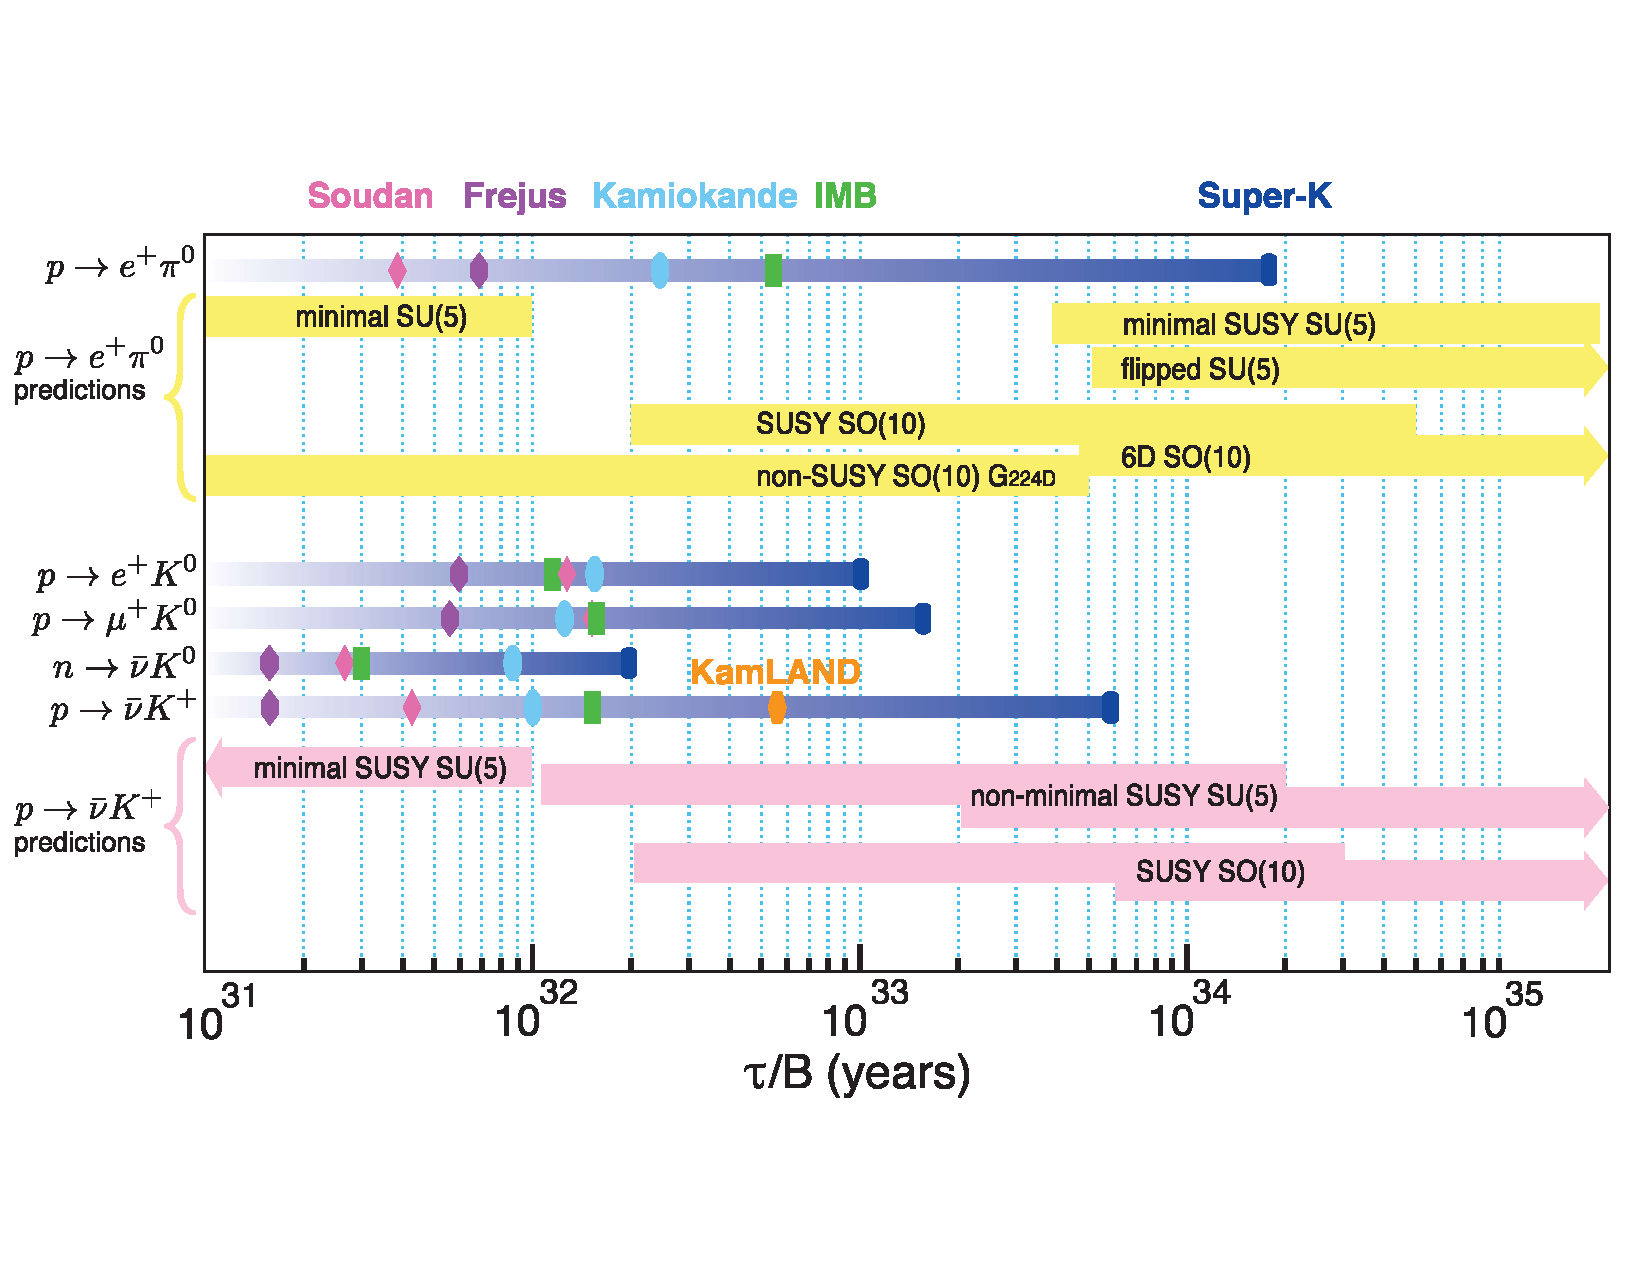
\includegraphics[width=0.9\textwidth]{TheoryExpLimitSummary.pdf}
\end{dunefigure}

\subsection{Experimental Signatures for Nucleon Decay Searches in DUNE}
\label{subsec:nonaccel-ndk-dune}

The \dword{dune} \dword{fd}, with the largest active volume of \dword{lar}, 
will be highly sensitive to several possible nucleon decay modes, 
in many cases complementing the capabilities of large water detectors.
In particular, \dword{lartpc} technology offers the opportunity to observe the entire decay chain for nucleon decays into charged kaons; in \ptoknubar, the kaon is typically below \cherenkov threshold in a water \cherenkov detector, but can be identified by its distinctive $dE/dx$ signature as well as by its decay in a \dword{lartpc}.
Therefore, this mode can be tagged in a \dword{lartpc} if a single kaon within a proper energy/momentum range can be reconstructed with its point of origin lying within the fiducial volume followed by a known decay mode of the kaon.
Background events initiated by cosmic-ray muons can be controlled  by requiring no activity close to the edges of the \dwords{tpc} and by stringent single kaon identification within the energy range of interest~\cite{bib:docdb3384,bib:docdb1752}.  Atmospheric neutrinos make up the dominant background.

Because of the already stringent limits set by \superk on \ptoepizero and the unique ability to track and identify kaons in a \dword{lartpc}, the initial nucleon decay studies in \dword{dune} have focused on nucleon decay modes featuring kaons.  Studies of \ptoepizero have begun (see Section~\ref{subsec:nonaccel-ndk-other}) but are less advanced than the kaon studies.  The remainder of this section describes the background assumptions, signal simulation, particle tracking and identification, and event classification with a focus on nucleon decay involving kaons.

\subsubsection{Background Simulation}
\label{sec:ndkbkgd}

The main background for nucleon decay searches is in the interactions of  atmospheric neutrinos. In this analysis, the Bartol model of atmospheric neutrino flux~\cite{Barr:2004br} is used.
Neutrino interactions in argon are simulated with the \dword{genie} event generator~\cite{Andreopoulos:2009rq}. To estimate the event rate, we integrate the product of the neutrino flux and interaction cross section.
Table \ref{tab:rate} shows the event rate for different neutrino species for an exposure of \SI{10}{\ktyr}, where oscillation effects are not included.

\begin{dunetable}
[Expected rate of atmospheric neutrino interactions]
{cccc}
{tab:rate}
{Expected rate of atmospheric neutrino interactions in \argon40 for a \SI{10}{\ktyr} exposure (not including oscillations).}
  ~\SI{10}{\ktyr}~   &~CC~&~NC~&~Total \\
\numu & \num{1038} & \num{398} &\num{1436} \\
\anumu &\num{280} & \num{169} & \num{449} \\
\nue & \num{597} &  \num{206} &\num{803} \\
\anue & \num{126} & \num{72} & \num{198} \\
Total & \num{2041} & \num{845} & \num{2886} \\
\end{dunetable}


Thus, to suppress atmospheric neutrino background to the level of one event per \si{\Mtyr}, which would yield \num{0.4} events after ten years of operation with a \SI{40}{\kt} fiducial volume, the necessary background rejection is $1 - (1/288600) = 1 - 3\times10^{-6} = 0.999997$, where background rejection is defined as the fraction of background that is not selected.

\subsubsection{Nucleon Decay Simulation}
\label{sec:ndksim}

The simulation of nucleon decay events is performed using GENIE v.2.12.10. 
A total of \num{68} single-nucleon exclusive decay channels listed in the 2016 update of the \dword{pdg}~\cite{Tanabashi:2018oca} %Patrignani:2016xqp} 
is available in \dword{genie} (see Table~\ref{tab:genie_ndk}). 
%in Appendix~\ref{sec:tools-app-generator}). 
The list includes two-, three-, and five-body decays. 
If a bound nucleon decays, the remaining nucleus can be in an excited state and will typically de-excite by emitting nuclear fission fragments, nucleons, and photons. At present, de-excitation photon emission is simulated only for oxygen~\cite{Andreopoulos:2015wxa}.  However, the \argoneut collaboration~\cite{Acciarri:2018myr} has reported measurements of argon de-excitation photons in \dword{lartpc} detectors,
where energy depositions and positions of these depositions have been compared to those from simulations of neutrino-argon interactions using the FLUKA Monte Carlo generator.  


\begin{table} % Anne leaving as is
  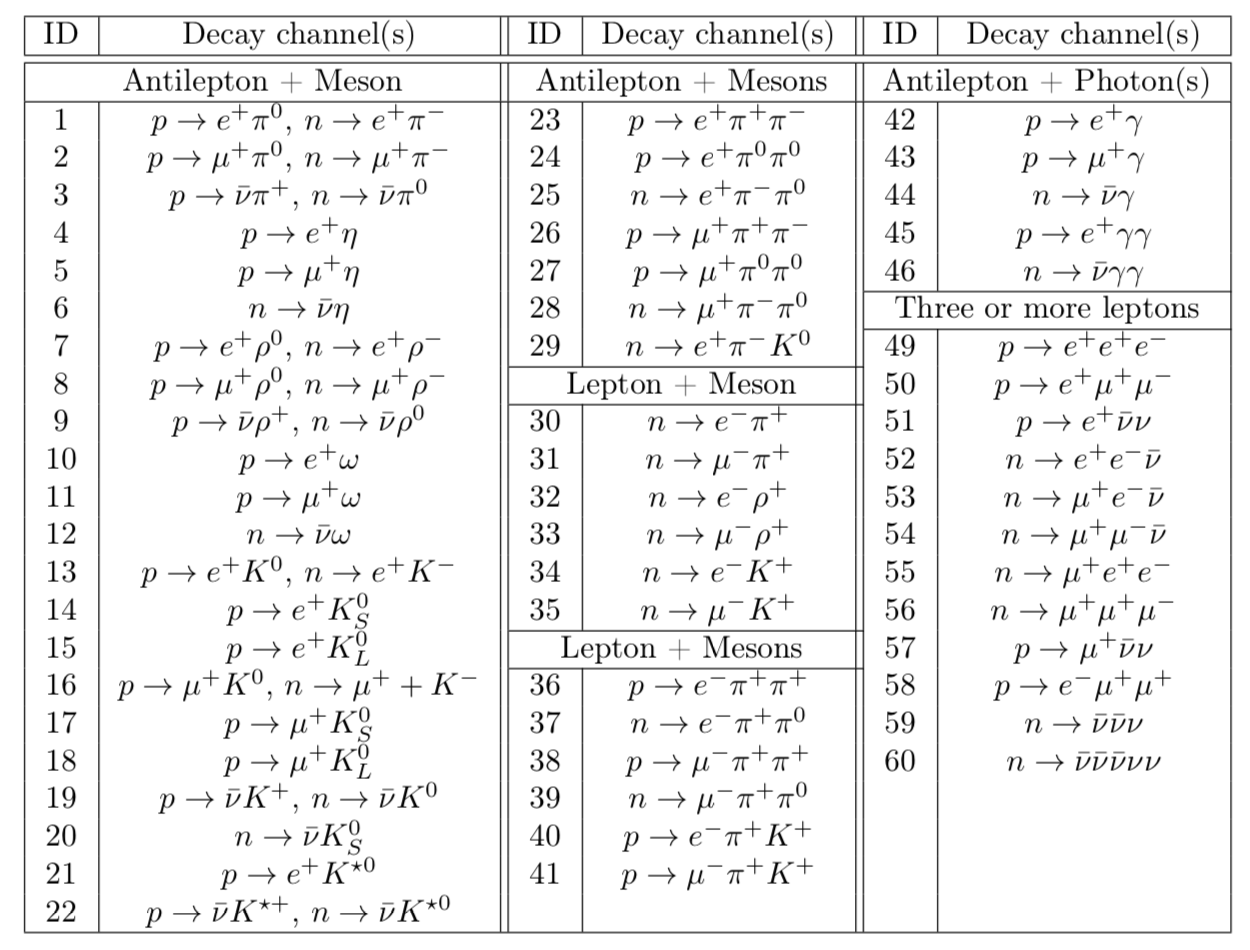
\includegraphics[width=\linewidth]{costas_table1}
  \caption[GENIE nucleon decay topologies]{Decay topologies considered in \dword{genie} nucleon decay simulation.}
  \label{tab:genie_ndk}
\end{table}


\subsubsection{Kaon Final State Interactions}
\label{sec:final-state-interactions}

The propagation of the decay products in the nucleus is simulated using an intranuclear cascade \dword{mc}. 
Charged kaons can undergo various scattering processes in the nucleus: elastic scattering, charge exchange, absorption (only $K^{-}$; $K^{+}$ absorption is forbidden), and $K^{+}$ production via strong processes such as $\pi^{+}n \rightarrow K^{+} \Lambda$.  In this analysis, the $hA2015$ model in \dword{genie} is used as the default model for these \dword{fsi}.  $hA2015$ is an empirical, data-driven method that does not model the cascade of hadronic interactions step by step, but instead uses one effective interaction where hadron+nucleus data is used to determine the final state.
For kaons, $K^{+}+C$ data~\cite{Bugg:1968zz,Friedman:1997eq}
is used when available. $hA2015$ only considers kaon-nucleon elastic scattering inside the nucleus.  Charge exchange is not included, nor is $K^+$ production in pion reactions, and therefore a $K^+$ is never added or removed from the final state in this model. 

Other \dword{fsi} models include the full cascade, but there is not enough data to favor one model over the other.  As an example of the limitations of the current data on kaon \dword{fsi}, a recent measurement of kaon production in neutrino interactions shows only a weak preference for including \dword{fsi} as opposed to a model with no \dword{fsi}~\cite{Marshall:2016rrn}.  In this case, the kaon \dword{fsi} have a relatively subtle effect on the differential cross section, and the available statistics are not sufficient to conclusively prefer one model over another.  For nucleon decay into kaons, the \dword{fsi} have a much larger impact, and the differences between models are less significant than the overall effect.  Kaon \dword{fsi} introduce an important uncertainty that is included in this analysis.

\dword{fsi} can significantly modify the observable distributions in the detector.  For example, Figure~\ref{fig:K-wFSI-hA2015} shows the kinetic energy of a kaon from \ptoknubar before and after \dword{fsi}. Because of \dword{fsi} the kaon spectrum becomes softer on average. Of the kaons, \num{31.5}\%  undergo elastic scattering resulting in events with very low kinetic energy;  \num{25}\% of kaons have a kinetic energy of $\le\SI{50}{\MeV}$. When the kaon undergoes elastic scattering, a nucleon can be knocked out of the nucleus. Of decays via this channel, \num{26.7}\%  have one neutron coming from \dword{fsi}, \num{15.3}\% have at least one proton, and \num{10.3}\% have two protons coming from \dword{fsi}. These secondary nucleons are detrimental to reconstructing and selecting  $K^{+}$.

\begin{dunefigure}[Kaon kinetic energy before and after final state interactions]{fig:K-wFSI-hA2015}{Kinetic energy of kaons in simulated proton decay events, \ptoknubar.  The kinetic energy distribution is shown before and after final state interactions in the argon nucleus.}
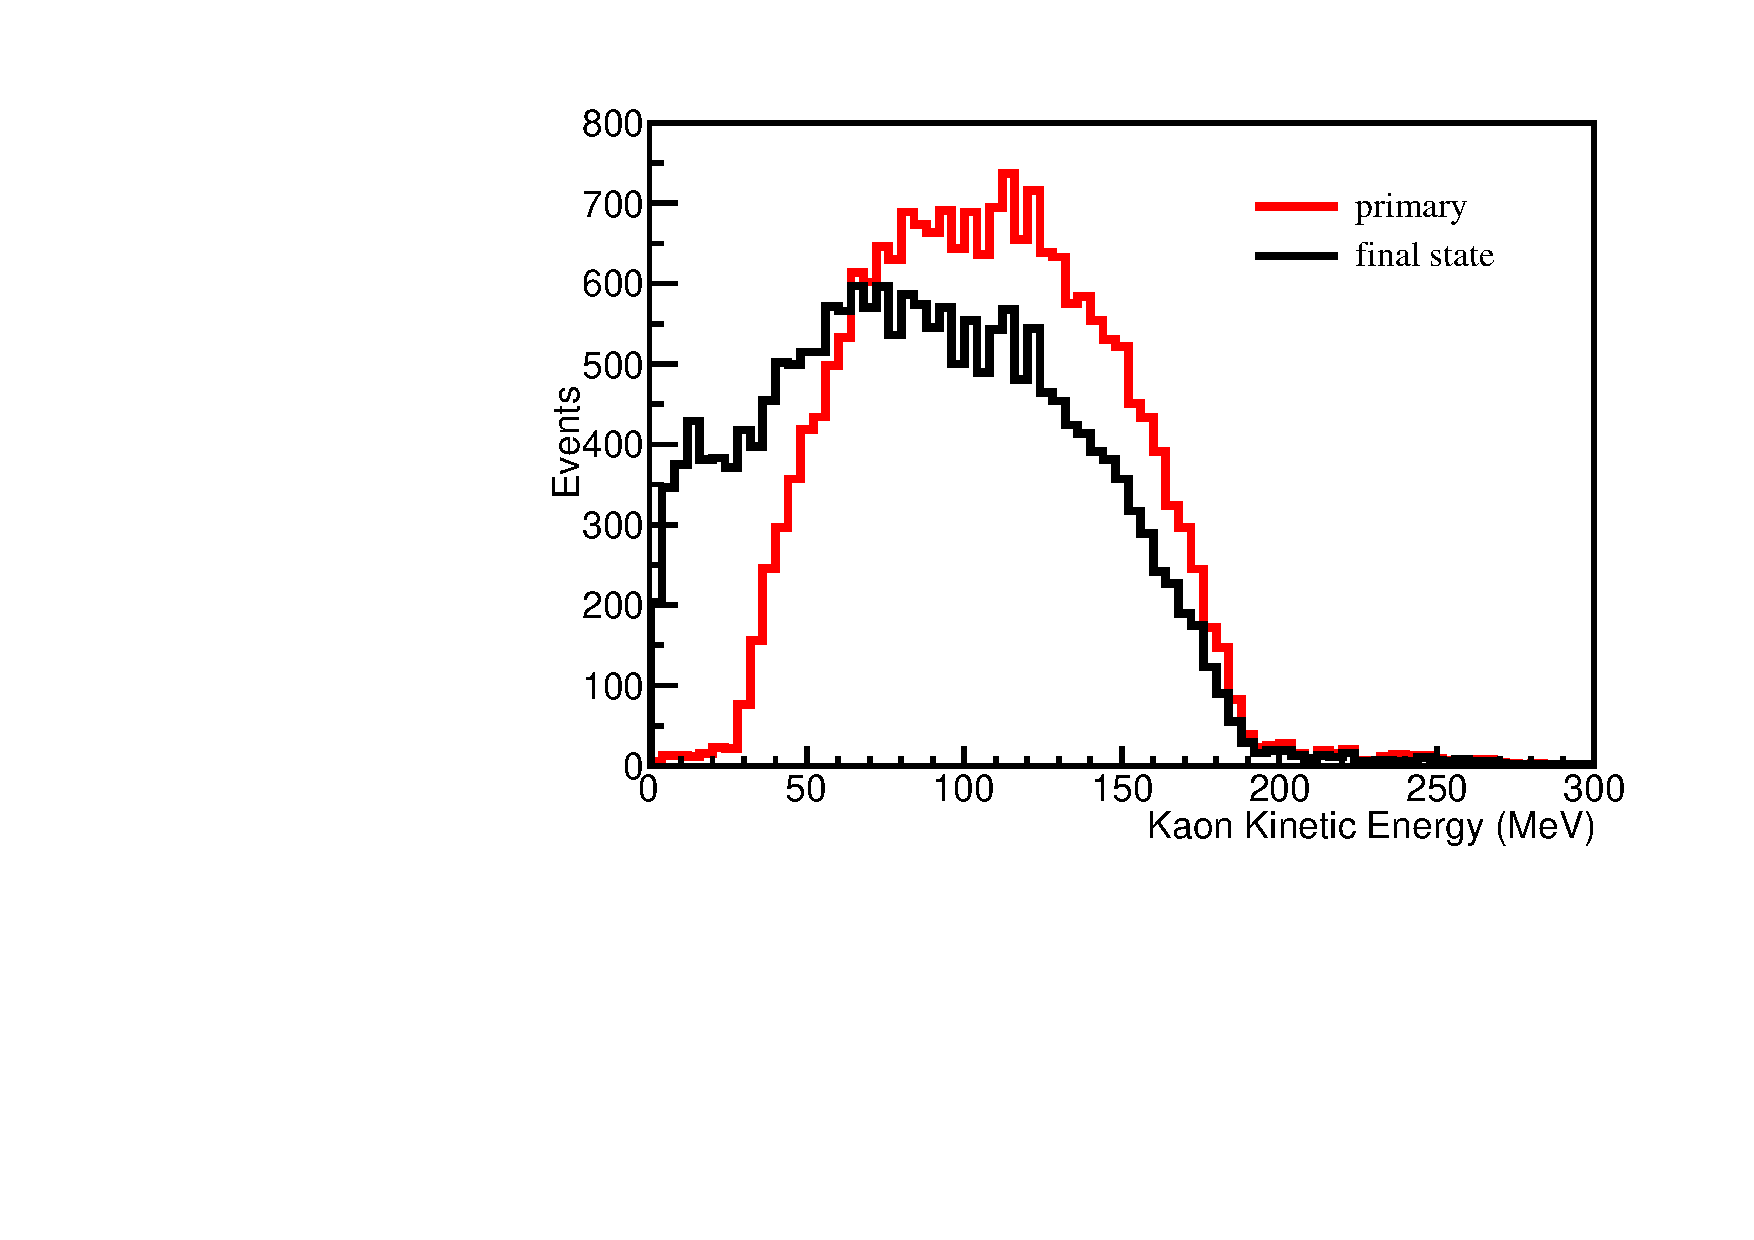
\includegraphics[width=0.8\textwidth]{K-wFSI-hA2015.pdf}
\end{dunefigure}

The kaon \dword{fsi} in \superk's simulation of \ptoknubar in oxygen seem to have a smaller effect on the outgoing kaon momentum distribution~\cite{Abe:2014mwa} than is seen here with the \dword{genie} simulation on argon.  Some differences are expected due to the different nuclei, but differences in the \dword{fsi} models are under investigation.

\subsubsection{Tracking and Particle Identification}
\label{sec:event-reconstruction}

The \dword{dune} reconstruction algorithms are described in Chapter~\ref{ch:tools}.  This analysis uses \threed track and vertex reconstruction provided by \dword{pma}.

Track reconstruction efficiency for a charged particle $x^{\pm}$ is defined as 
\begin{equation}
\epsilon_{x^{\pm}} = \frac{\mbox{$x^{\pm}$ particles with a reconstructed track}}{\mbox{events with $x^{\pm}$ particle }}.
\end{equation}
The denominator includes events in which an $x^{\pm}$ particle was created and has deposited energy within any of the \dwords{tpc}.  The numerator includes events in which an $x^{\pm}$ particle was created and has deposited energy within any of the \dwords{tpc}, and a reconstructed track can be associated to the $x^{\pm}$ particle based on the number of hits generated by that particle along the track. This efficiency can be calculated as a function of true kinetic energy and true track length.

\begin{dunefigure}[Tracking efficiency of kaons in \ptoknubar]{fig:k-trk-eff}{Tracking efficiency for kaons in simulated proton decay events, \ptoknubar, as a function of kaon kinetic energy (left) and true path length (right).}
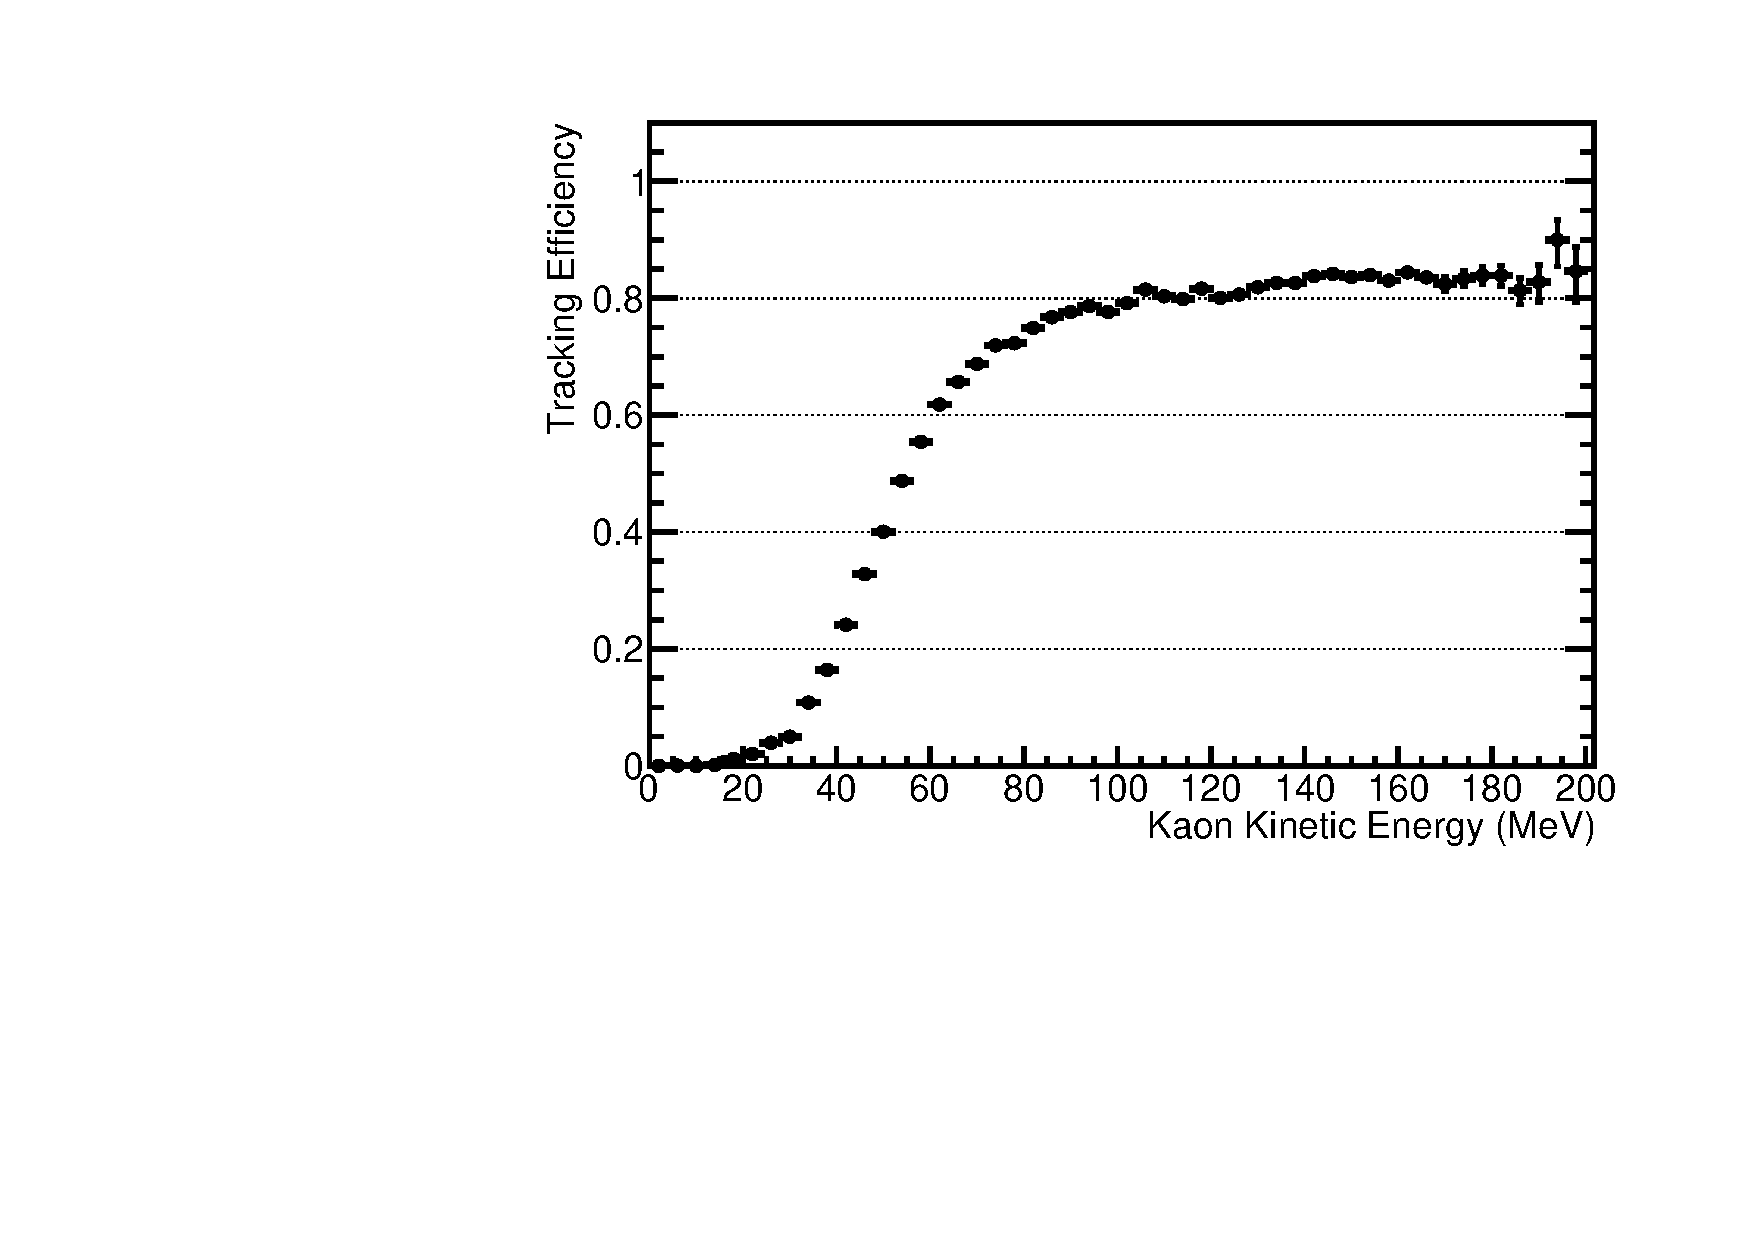
\includegraphics[width=0.4\textwidth]{k-trk-eff-KE.pdf}
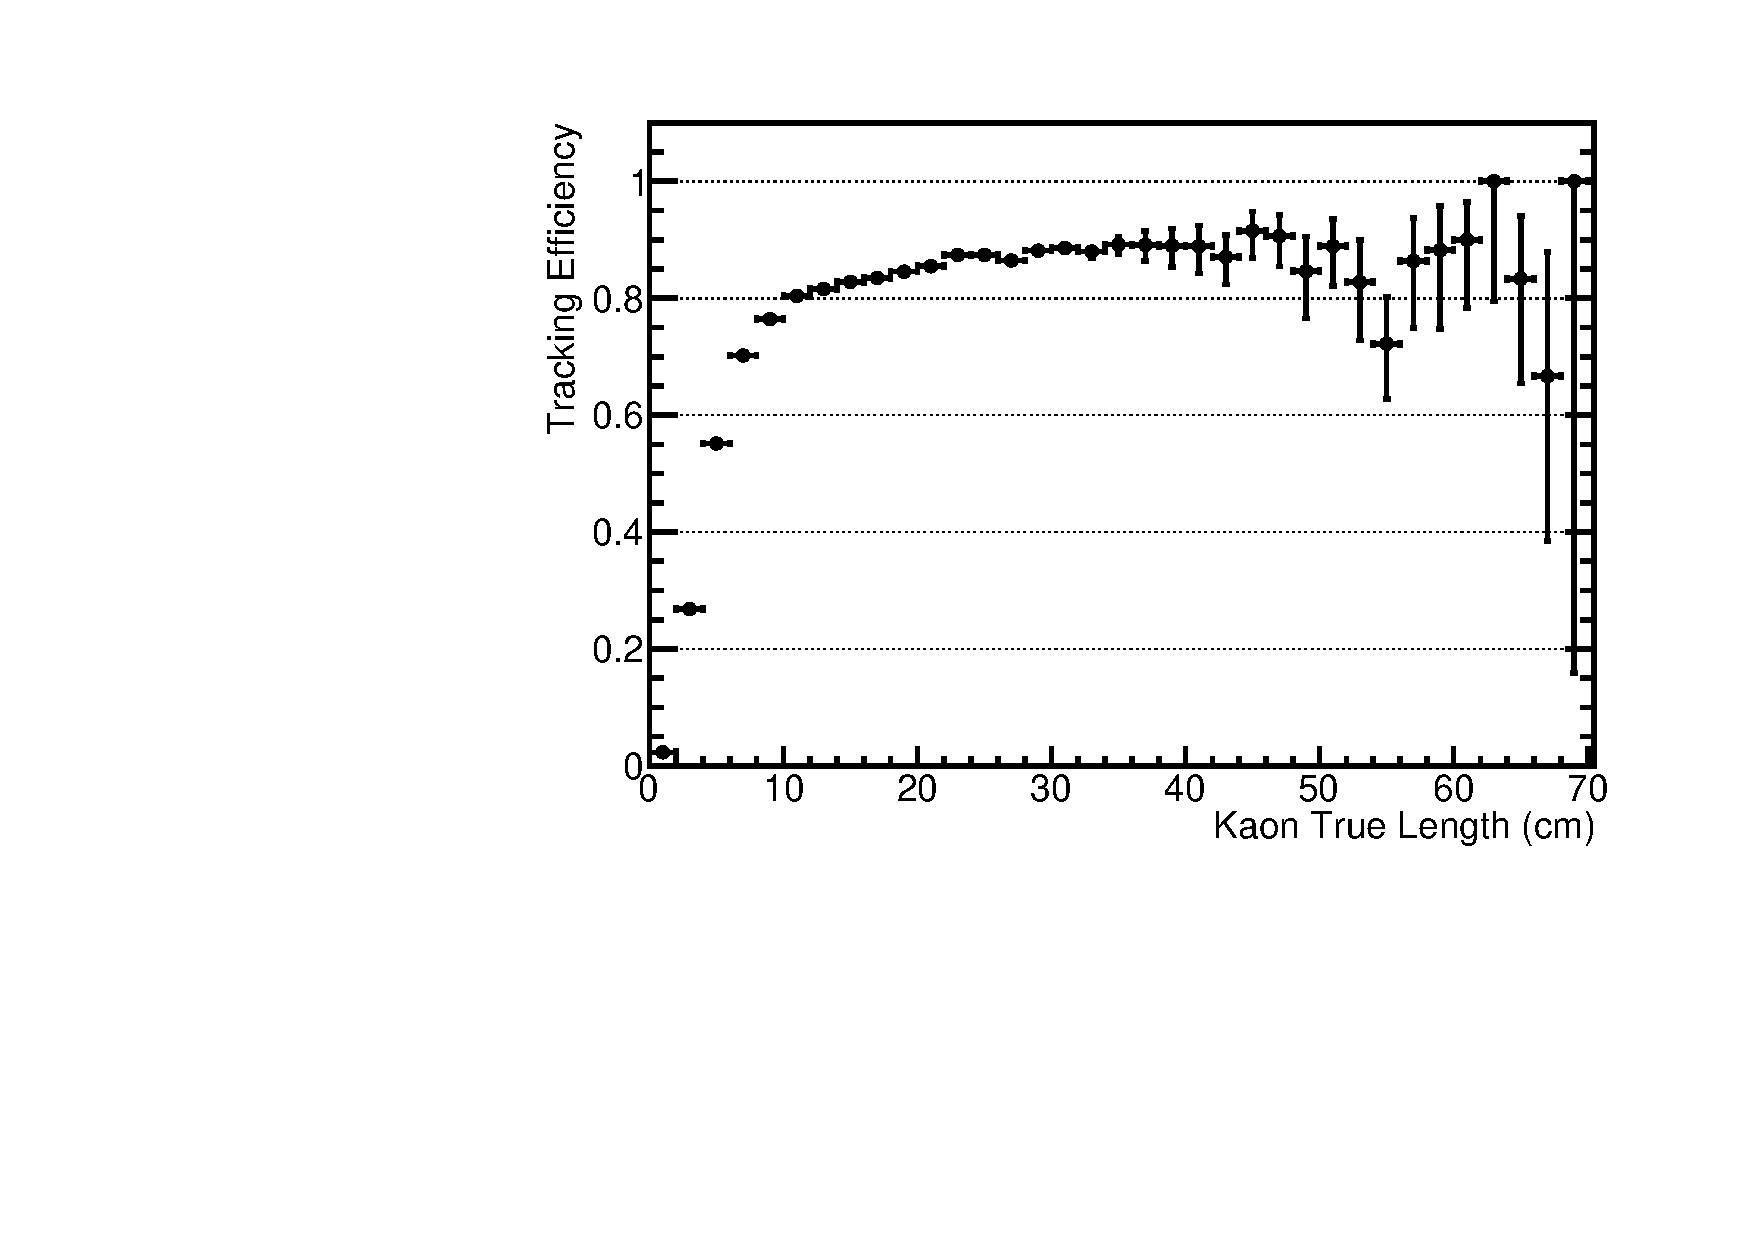
\includegraphics[width=0.4\textwidth]{k-trk-eff-length.pdf}
\end{dunefigure}

Figure~\ref{fig:k-trk-eff} shows the tracking efficiency for $K^{+}$  from proton decay via \ptoknubar as a function of true kinetic energy and true path length. The overall tracking efficiency for kaons is \num{58.0}\%, meaning that \num{58.0}\% of all the simulated kaons are associated with a reconstructed track in the detector.  From Figure~\ref{fig:k-trk-eff}, the tracking threshold is approximately $\sim\SI{40}{\MeV}$ of kinetic energy, which translates to $\sim\SI{4.0}{\cm}$ in true path length.  The biggest loss in tracking efficiency is due to kaons with $<\SI{40}{\MeV}$ of kinetic energy due to scattering inside the nucleus as described in Section~\ref{sec:final-state-interactions}.  The efficiency levels off to approximately \num{80}\% above \SI{80}{\MeV} of kinetic energy.  This inefficiency even at high kinetic energy is due mostly to kaons that decay in flight./footnote{No attempt has been made at this point to recover such events.}
Both kaon scattering in the \dword{lar} and charge exchange are included in the simulation but are relatively small effects (\num{4.6}\% of kaons scatter in the \dword{lar} and \num{1.2}\% of kaons experience charge exchange).   The tracking efficiency for muons from the decay of the $K^{+}$ in \ptoknubar is \num{90}\%.

Charged particles lose energy through ionization and scintillation when traversing the \dword{lar}. This energy loss provides valuable information on particle energy and species. To identify a given particle, the hits associated with a reconstructed track are used.
%The total energy deposition from the track is obtained by summing the $dE/dx$ for all reconstructed hits. 
If the charged particle stops in the \dword{lartpc} active volume, a combination of $dE/dx$ and the reconstructed residual range ($R$, the path length to the end point of the track) is used to define a parameter for \dword{pid}.  The parameter, $PIDA$, %\fixme{This abbreviation (PIDA) is not in the glossary. There is a PID, which is apparently what you mean here.} 
%PIDA is a variable name, not an abbreviation.  PIDA is a variable that is used to perform particle identification (PID).  I put PIDA in math mode, like dE/dx, to make that clear.
is defined as~\cite{Acciarri:2013met}  
%
\begin{equation}
PIDA = \left\langle \left(\frac{dE}{dx}\right)_{i}R^{0.42}_{i}\right\rangle,\label{eqn:PIDA}
\end{equation}
where the median is taken over all track points $i$ for which the residual range $R_i$ is less than \SI{30}{\cm}.

\begin{dunefigure}[Particle identification using $PIDA$ for \ptoknubar]{fig:PIDA}{Particle identification using $PIDA$ for muons and kaons in simulated proton decay events, \ptoknubar, and protons in simulated atmospheric neutrino background events.  The curves are normalized by area.}
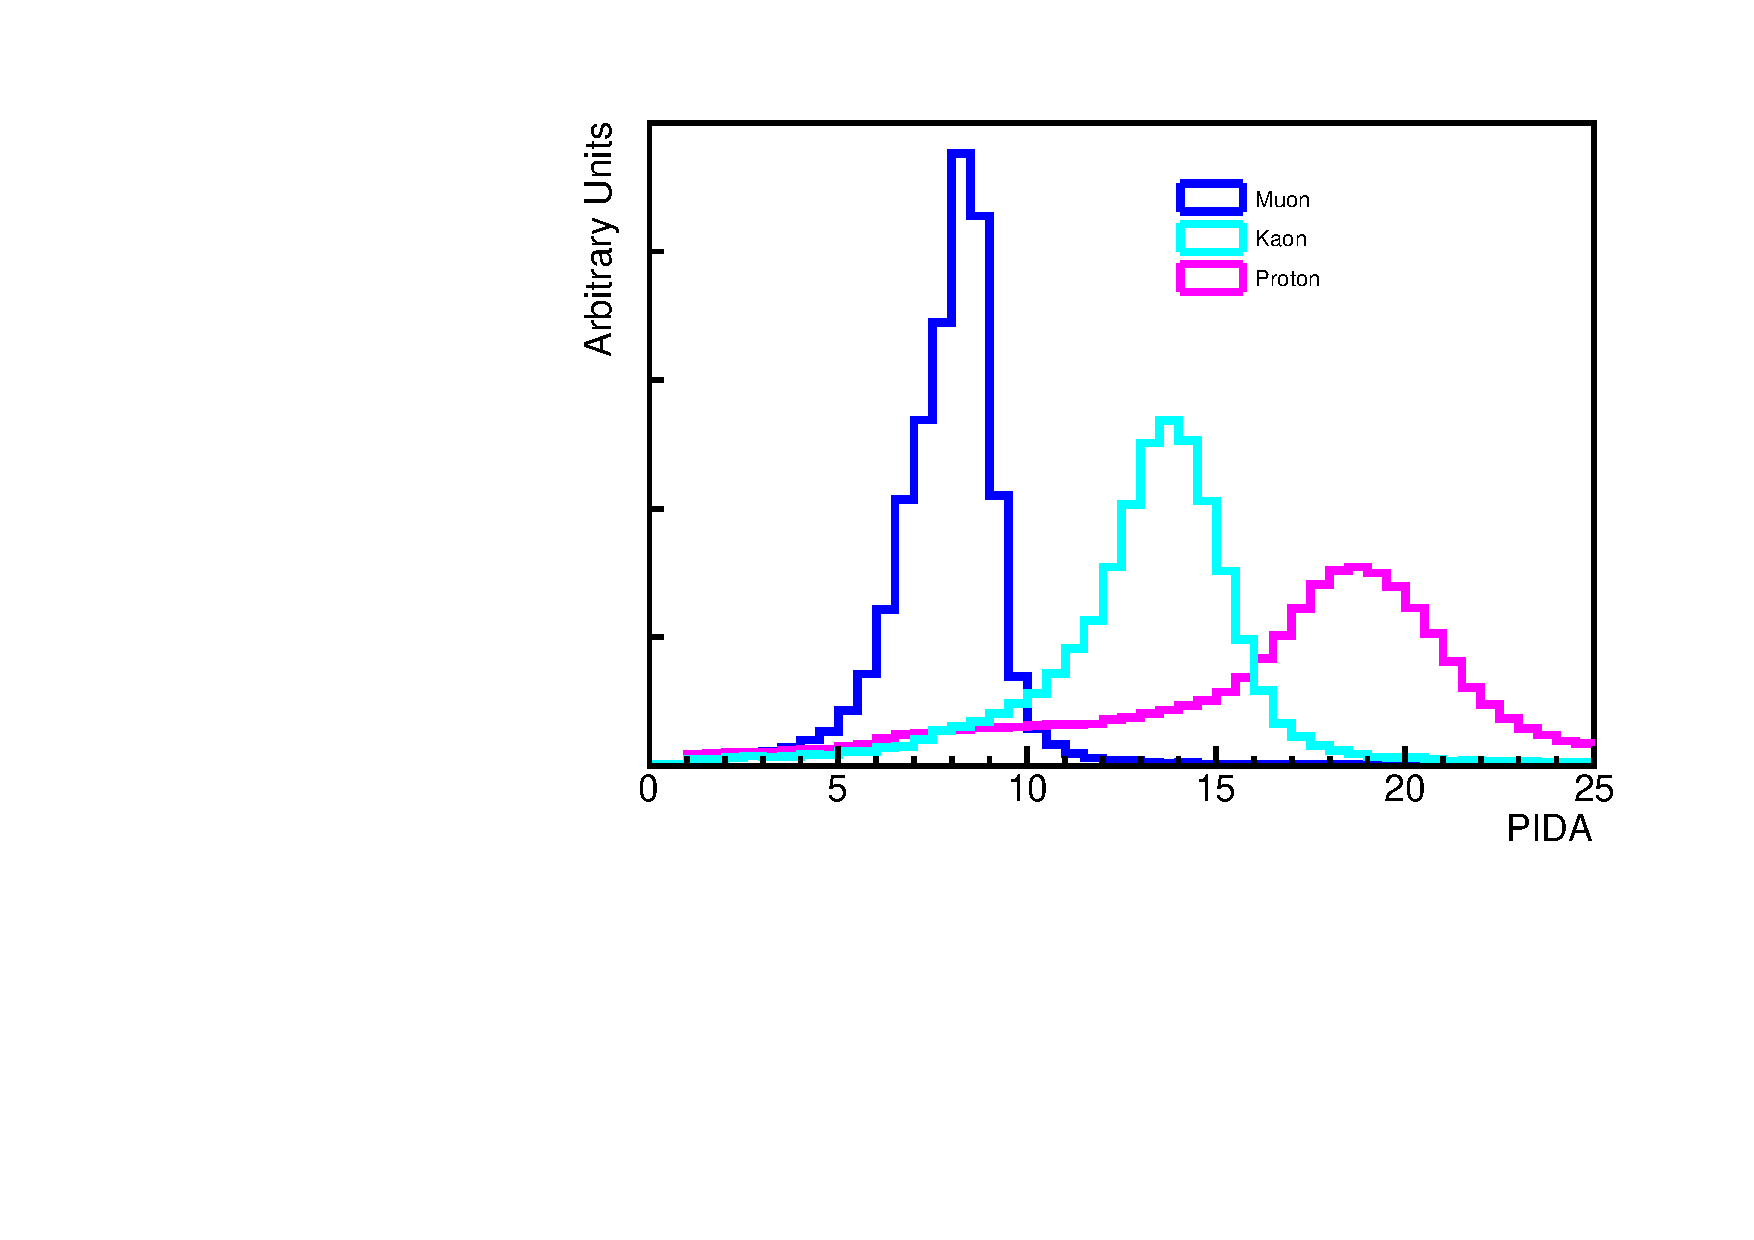
\includegraphics[width=0.8\textwidth]{PIDA.pdf}
\end{dunefigure}

Figure~\ref{fig:PIDA} shows the $PIDA$ performance for kaons (from proton decay), muons (from kaon decay), and protons produced by atmospheric neutrino interactions. The tail with lower values in each distribution is due to cases where the decay/stopping point was missed by the track reconstruction. The tail with higher values is caused when a second particle overlaps at the decay/stopping point causing higher values of $dE/dx$ and resulting in higher values of $PIDA$. In addition, ionization fluctuations smear out these distributions.

A complication for \dword{pid} via $dE/dx$ results when ambiguity occurs in reconstructing track direction, which is even more problematic because additional energy deposition may occur at the originating point in events where \dword{fsi} is significant.  The dominant background to \ptoknubar in \dword{dune} is atmospheric neutrino \dword{cc} \dword{qe}
scattering, $\nu_{\mu} n \rightarrow \mu^{-} p$.  When the muon happens to have very close
to the \SI{237}{\MeV$/c$} momentum expected from a $K^{+}$ decay at rest and does not capture, it is indistinguishable from the muon resulting from \ptoknubar followed by $K^{+} \rightarrow \mu^{+}\nu_{\mu}$. When
the proton is also mis-reconstructed as a kaon, this background mimics the signal process.  

The most important difference between signal and this background source is the direction of the hadron track. For an atmospheric neutrino, the proton and muon originate from the same neutrino interaction point, and the characteristic Bragg rise occurs at the end of the proton track farthest from the muon-proton vertex. For signal, the kaon-muon vertex location is where the $K^{+}$ stops and decays at rest, so its ionization energy deposit is highest near the kaon-muon vertex.  To take advantage of this difference, a log-likelihood ratio discriminator is used to distinguish signal from background.  Templates are formed by taking the reconstructed and calibrated energy deposit as a function of the number of wires from both the start and end of the $K^{+}$ candidate hadron track. 
%The best view is used, which is typically the collection plane. 
Two log-likelihood ratios are computed separately for each track. The first begins at the hadron-muon shared vertex and moves along the hadron track (the ``backward'' direction). The second begins at the other end of the track, farthest from the hadron-muon shared vertex, moves along the hadron track the other way (the ``forward'' direction). For signal events, this effectively looks for the absence of a Bragg rise at the $K^{+}$ start, and the presence of one at the end, and vice versa for background.  At each point, the probability density for signal and background, $P^{sig}$ and $P^{bkg}$, are determined from the templates. Forward and backward log-likelihood ratios are computed as
%
\begin{align}
 \mathcal{L}_{fwd(bkwd)} = \sum_{i} \log\frac{P^{sig}_i}{P^{bkg}_i}, 
\end{align}
where the summation is over the wires of the track, in either the forward or backward direction.  Using either the forward or backward log-likelihood ratio alone gives some discrimination between signal and background, but using the sum gives better discrimination. While the probability densities are computed based on the same samples, defining one end of the track instead of the other as the vertex provides more information. The discriminator is the sum of the forward and backward log-likelihood ratios:
%
\begin{align}
    \mathcal{L} = \mathcal{L}_{fwd} + \mathcal{L}_{bkwd}.\label{eqn:L}
\end{align}
Applying this discriminator to tracks with at least ten wires gives a signal efficiency of roughly \num{0.4} with a background rejection of \num{0.99}.

\subsubsection{Event Classification}

Multivariate classification methods based on machine learning techniques have become a fundamental part of most analyses in high-energy physics. 
To develop an event selection to search for nucleon decay, a \dword{bdt}
classifier is used. The software package Toolkit for Multivariate Data Analysis with ROOT (TMVA4)~\cite{Hocker:2007ht}
was used with AdaBoost as the boosted algorithm.  In the analyses presented here, the \dword{bdt} is trained on a sample of \dword{mc} events (\num{50000} events for signal and background) that is statistically independent from the sample of \dword{mc} events used in the analysis (approximately \num{100000} events for signal and \num{600000} events for background.)  This technique is used for the nucleon decay and neutron-antineutron analyses presented below.

As an independent method of identifying nucleon decay events, image classification using a \dword{cnn}
can be performed using \twod images of \dword{dune} \dword{mc} events. The image classification provides a single score value as a metric of whether any given event is consistent with a proton decay, and this score can be used as a powerful discriminant for event identification.  In the analyses presented here, the \dword{cnn} technique alone does not discriminate between signal and background as well as a \dword{bdt}.  For that reason, the \dword{cnn} score is used as one of the input variables in the \dword{bdt} in each analysis.

\subsection{Sensitivity to \ptoknubar Decay}
\label{subsec:nonaccel-ndk-nubarkplus}

Monte Carlo studies of the \ptoknubar signal and corresponding atmospheric neutrino backgrounds have been carried out with the \dword{dune} multipurpose full event simulation and reconstruction software.  As indicated in Section~\ref{sec:event-reconstruction},
they reveal that one of the main challenges in identifying proton decay candidates is suppressing backgrounds arising from the mis-reconstruction of protons as positive kaons. This happens when a \dword{cc} neutrino interaction produces a muon and a recoiling proton, and the primary vertex for neutrino interaction is mislabeled as a secondary vertex where the kaon decays.  Complicating the ability to reject pathological events of this type is the presence of \dword{fsi}, which can shift the spectrum of kaons toward low energies, with possible concurrent emission of nucleons, which together weaken the otherwise distinct energy and $dE/dx$ signature of the kaon. 

The branching fraction for leptonic decay of charged kaons, $K\rightarrow \mu \nu_{\mu}$, is approximately \num{64}\%. The remaining decay modes are semileptonic or hadronic and include charged and neutral pions. The leptonic decay offers a distinguishable topology with a heavy ionizing particle followed by a minimum ionizing particle. In addition, given the kinematics of a proton decay event, \num{92}\% of kaons decay at rest. Using two-body kinematics, the momentum of the muon is approximately \SI{237}{\MeV$/c$}. The reconstructed momentum of the muon offers a powerful discriminating variable to separate signal from background events.  This analysis includes all modes of kaon decay, but the selection strategy so far has focused on kaon decay to muons.

The proton decay signal and atmospheric neutrino background events are processed using the same reconstruction chain and subject to the same selection criteria. There are two pre-selection cuts to remove obvious background. One cut requires at least two tracks, which aims to select events with a kaon plus a kaon decay product (usually a muon).  The other cut requires that the longest track be less than \SI{100}{\cm}; this removes backgrounds from high energy neutrino interactions.  After these cuts, \num{50}\% of the signal and \num{17.5}\% of the background remain in the sample.  The signal inefficiency at this stage of selection is due mainly to the kaon tracking efficiency.

A \dword{cnn} was developed to classify signal and background events that gives \num{99.9}\% background rejection at \num{6}\% signal efficiency.  Better discriminating power is achieved using a \dword{bdt} with \num{14} input variables, including the \dword{cnn} score as one  variable.  The other variables in the \dword{bdt} include numbers of reconstructed objects (tracks, showers, vertices), variables related to visible energy deposition, \dword{pid} variables ($PIDA$, Equation~\ref{eqn:PIDA}, and $\mathcal{L}$, Equation~\ref{eqn:L}), reconstructed track length, and reconstructed momentum.

Figure~\ref{fig:BDT_response} shows the distribution of the \dword{bdt} output for signal and background.

\begin{dunefigure}
[Boosted Decision Tree response for \ptoknubar ]{fig:BDT_response}
{Boosted Decision Tree response for \ptoknubar for signal (blue) and background (red).}
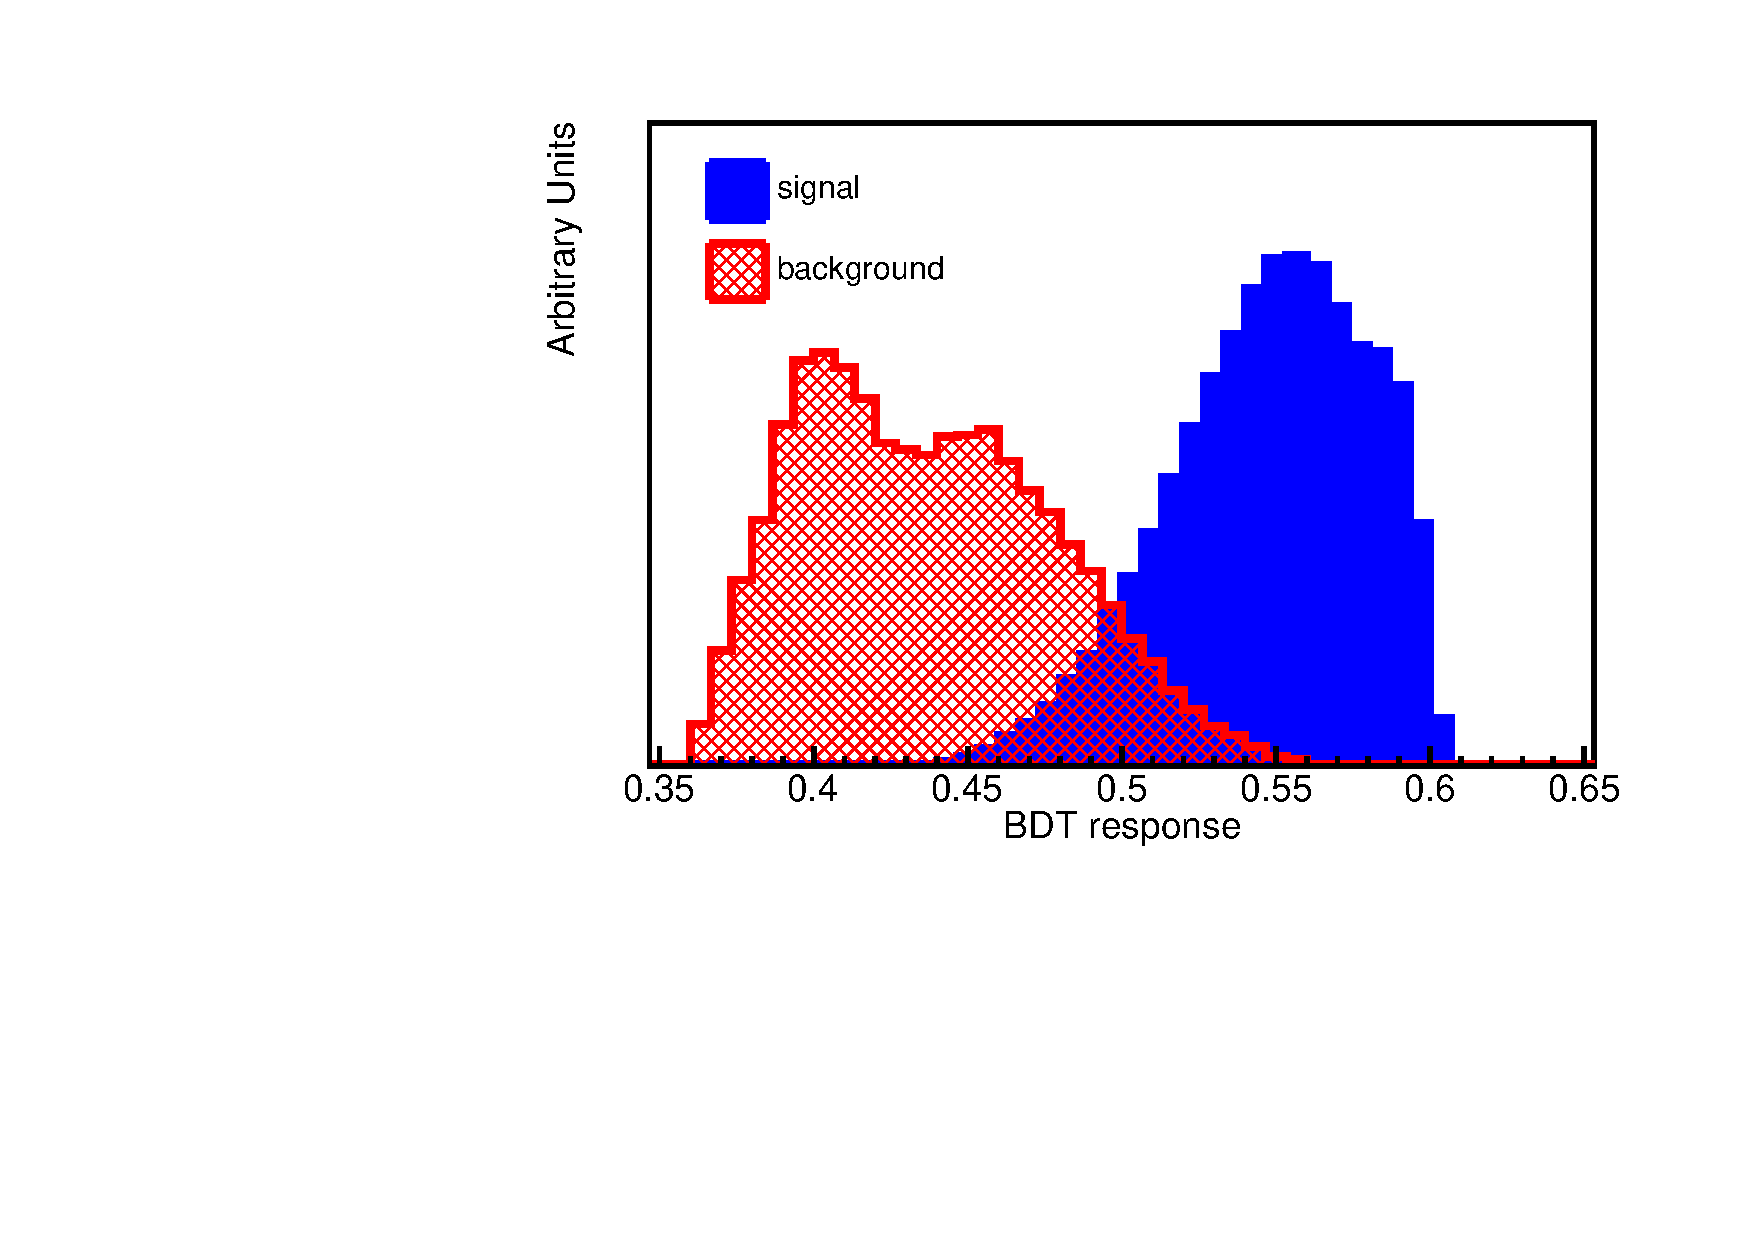
\includegraphics[width=0.8\textwidth]{BDT_response.pdf}
\end{dunefigure} 

Figure~\ref{fig:event_signal} shows a signal event with high \dword{bdt} response value (\num{0.605}), meaning a well-classified event. The event display shows the reconstructed kaon track in green, the reconstructed muon track from the kaon decay in maroon, and the reconstructed shower from the Michel electron coming from the muon decay in red. Figure~\ref{fig:event_bkgd} shows event displays for atmospheric neutrino interactions.  The left figure (\dword{bdt} response value of \num{0.394}) shows the interaction of an atmospheric electron neutrino, $\nu_{e}+n\rightarrow e^{-}+p+\pi^{0}$.  This event is clearly distinguishable from the signal.  However, the right figure (\dword{bdt} response value \num{0.587}) shows a \dword{cc}\dword{qe} interaction of an atmospheric muon neutrino, $\nu_{\mu}+n \rightarrow \mu^{-}+p$, which is more likely to be mis-classified as a signal interaction. These types of interactions present a challenge if the proton track is misidentified as kaon. A tight cut on \dword{bdt} response can remove most of these events, but this significantly reduces signal efficiency.


\begin{dunefigure}
[\ptoknubar signal event display]{fig:event_signal}
{Event display for a well-classified \ptoknubar signal event.  The vertical axis is time ticks (each time tick corresponds to \SI{500}{\ns}), and the horizontal axis is wire number. The bottom view is induction plane one, middle is induction plane two and top is the collection plane. The color represents the charge deposited in each hit.}
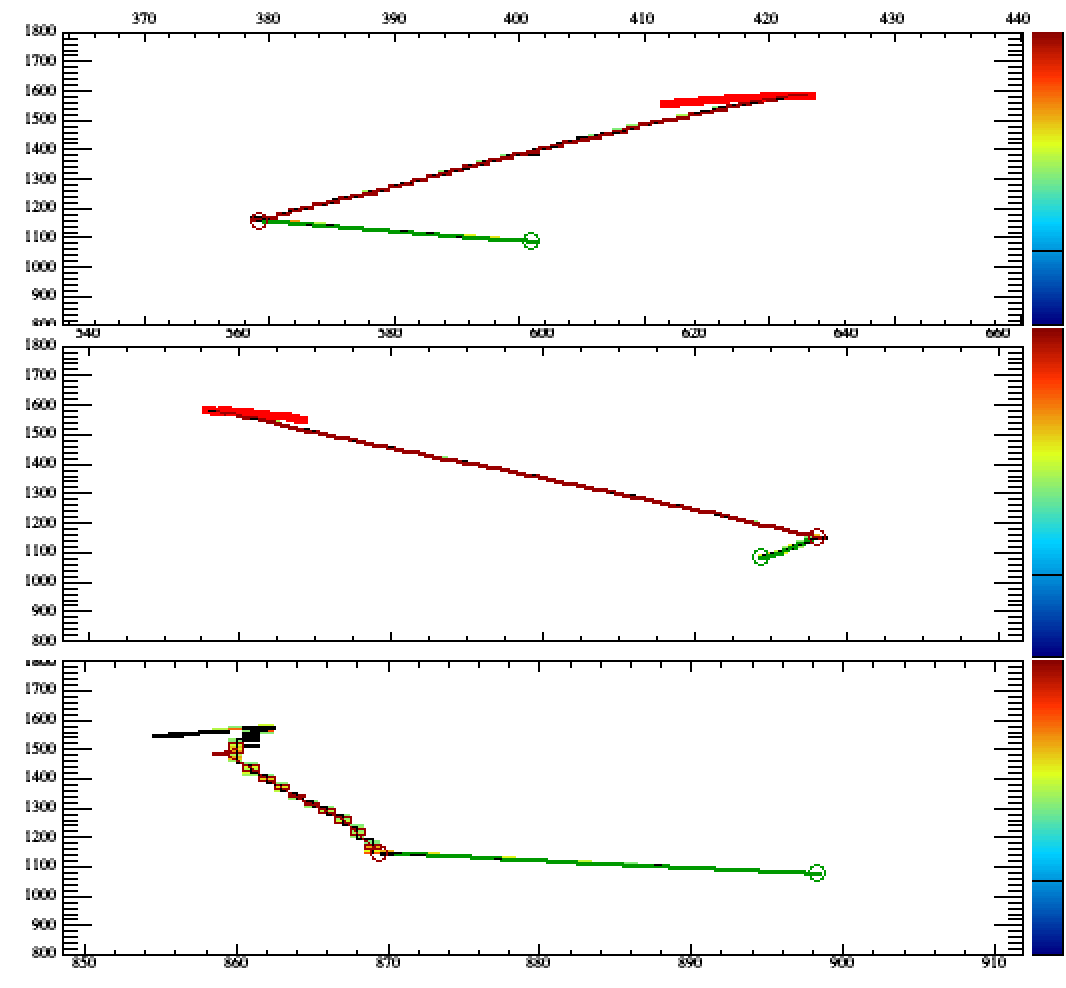
\includegraphics[width=0.8\textwidth]{event_signal.png}
\end{dunefigure} 

\begin{dunefigure}
[\ptoknubar background event displays]{fig:event_bkgd}
{Event displays for \ptoknubar backgrounds.  The vertical axis is time ticks (each time tick corresponds to \SI{500}{\ns}), and the horizontal axis is wire number. The bottom view is induction plane one, middle is induction plane two and top is the collection plane. The color represents the charge deposited in each hit. The left shows an atmospheric neutrino interaction unlikely to be classified as signal. The right shows an atmospheric neutrino interaction which could make it into the selected sample without a tight cut.}
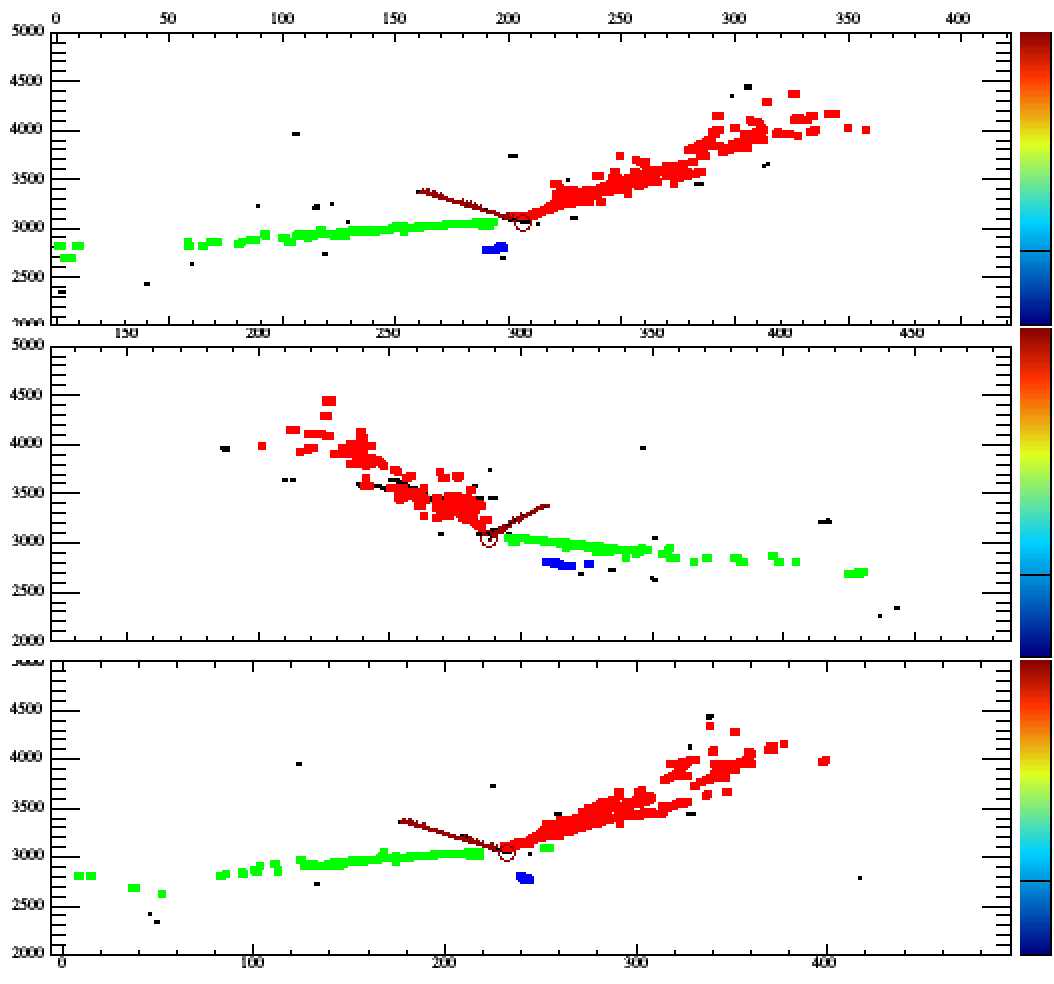
\includegraphics[width=0.48\textwidth]{event_bkgd_1.png}
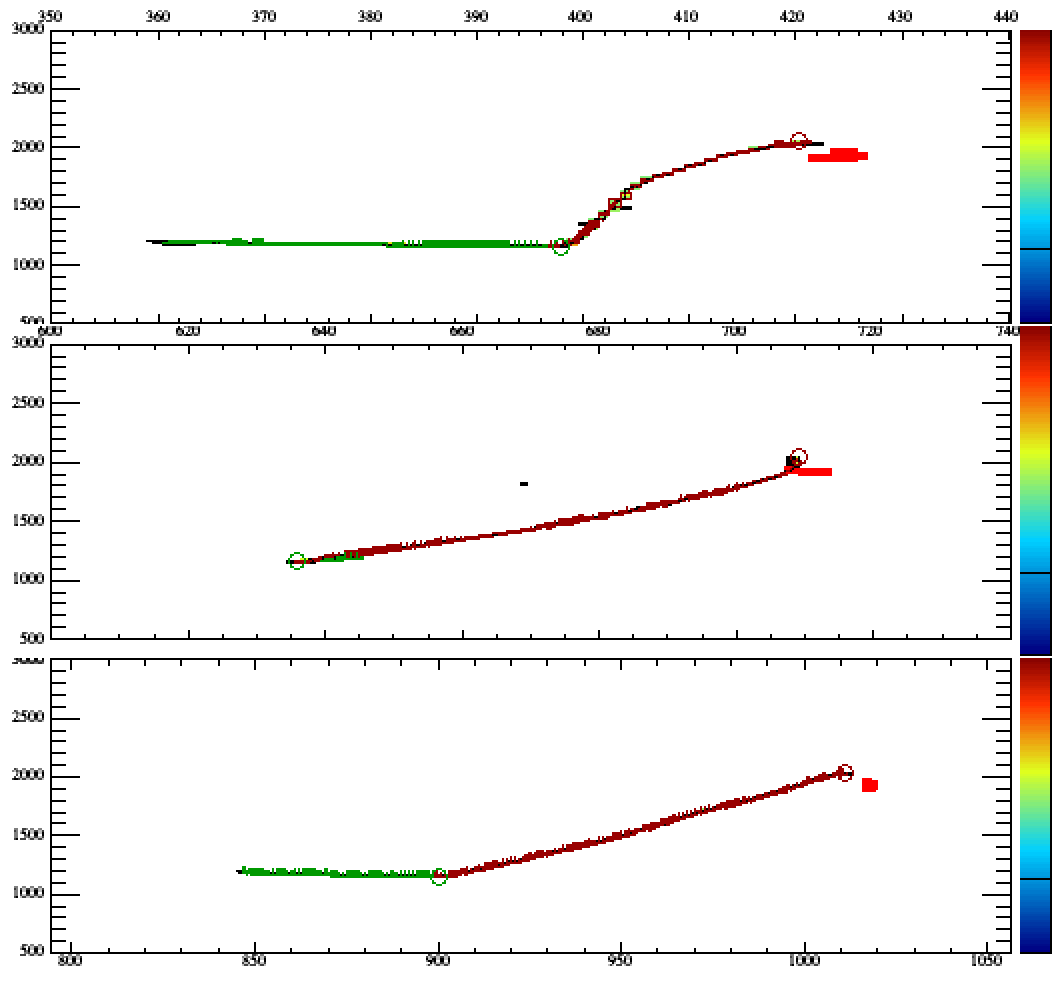
\includegraphics[width=0.48\textwidth]{event_bkgd_2.png}
\end{dunefigure}

Optimal lifetime sensitivity is achieved by combining the pre-selection cuts with a \dword{bdt} cut that gives a signal efficiency of \num{0.15} and a background rejection of 
$0.999997$,
%$1-3\times 10^{-6}$,
which corresponds to approximately one background event per \si{\Mtyr}. 
%Assuming no signal is observed over ten years of running with a total of \SI{40}{\kt} of fiducial mass, a \num{90}\% \dword{cl} lower limit on the proton lifetime in this channel of \SI{6.6e33}{\years} can be set. This calculation assumes constant signal efficiency and background rejection over time and for each of the \dword{fd} modules.  Additional running improves the sensitivity proportionately if the experiment remains background-free.

The limiting factor in the sensitivity is the kaon tracking efficiency.  With the current reconstruction, 
the overall kaon tracking efficiency is \num{58}\%.
The reconstruction is not yet optimized, and the kaon tracking efficiency should increase with improvements in the reconstruction algorithms.  
To understand the potential improvement, a visual scan of simulated decays of kaons into muons was performed. For this sample of events, with kaon momentum in the \SIrange{150}{450}{\MeV$/c$} range, scanners achieved greater than \num{90}\% efficiency at recognizing the $K^{+} \rightarrow \mu^{+} \rightarrow e^{+}$ decay chain.  The inefficiency came mostly from short kaon tracks (momentum below \SI{180}{\MeV$/c$}) and kaons that decay in flight. Note that the lowest momentum kaons ($<$\SI{150}{\MeV$/c$}) were not included in the study; the path length for kaons in this range would also be too short to track.  Based on this study, the kaon tracking efficiency could be improved to a maximum value of approximately \num{80}\% with optimized reconstruction algorithms, where the remaining inefficiency comes from low-energy kaons and kaons that charge exchange, scatter, or decay in flight.
Combining this tracking performance improvement with some improvement in the $K/p$ separation performance for short tracks, the overall signal selection efficiency improves from \num{15}\% to approximately \num{30}\%.
%This would double the sensitivity.

The analysis presented above is inclusive of all possible modes of kaon decay; however, the current version of the \dword{bdt} preferentially selects kaon decay to muons, which has a branching fraction of roughly \num{64}\%. The second most prominent kaon decay is $K^{+} \rightarrow \pi^{+}\pi^0$, which has a branching fraction of \num{21}\%.  Preliminary studies that focus on reconstructing a $\pi^{+}\pi^0$ pair with the appropriate kinematics indicate that the signal efficiency for kaons that decay via the $K^{+} \rightarrow \pi^{+}\pi^0$ mode is approximately the same as the signal efficiency for kaons that decay via the $K^{+} \rightarrow \mu^{+}\nu_{\mu}$ mode.  This assumption is included in our sensitivity estimates below.

The dominant systematic uncertainty in the signal is expected to be due to the kaon \dword{fsi}. To account for this uncertainty, kaon-nucleon elastic scattering ($K^{+}p(n)\rightarrow K^{+}p(n)$) is re-weighted by $\pm \num{50}\%$ in the simulation. 
The absolute uncertainty on the efficiency with this re-weighting is \num{2}\%, which is taken as the systematic uncertainty on the signal efficiency.
%The spread in signal efficiency with this re-weighting is $(15\pm 2)$\%, which is taken as the  systematic uncertainty on the signal efficiency.
The dominant uncertainty in the background 
is due to the absolute normalization of the atmospheric neutrino rate. The Bartol group has carried out a detailed study of the systematic uncertainties, where the absolute neutrino fluxes have uncertainties of approximately \num{15}\%~\cite{Barr:2006it}.
The remaining uncertainties are due to the cross section models for neutrino interactions.
The uncertainty on the \dword{cc}0$\pi$ cross section in the energy range relevant for these backgrounds is roughly \num{10}\%~\cite{Mahn:2018mai}.
%Uncertainty in the total neutrino \dword{cc} cross section peaks at \num{8}\% in the \SIrange{1}{5}{\GeV} region~\cite{Adamson:2012gt}.
Based on these two effects, a conservative \num{20}\% systematic uncertainty in the background is estimated.
%Finally a 0.1$\%$ uncertainty in the calculation of the fiducial volume is proposed. 

With a \num{30}\% signal efficiency and an expected background of one event per \si{\Mtyr}, a \num{90}\% \dword{cl} lower limit on the proton lifetime in the \ptoknubar channel of \SI{1.3e34}{years} can be set, assuming no signal is observed over ten years of running with a total of \SI{40}{\kt} of fiducial mass. This calculation assumes constant signal efficiency and background rejection over time and for each of the \dword{fd} modules.  Additional running improves the sensitivity proportionately if the experiment remains background-free.

\subsection{Sensitivity to Other Key Nucleon Decay Modes}
\label{subsec:nonaccel-ndk-other}

Another potential mode for a baryon number violation search is the decay of the neutron into a charged lepton plus meson, i.e.~\ntoek. In this mode, $\Delta B = -\Delta L$, where $B$ is baryon number and $L$ is lepton number.  The current best limit on this mode is \SI{3.2e31}{years} from the FREJUS collaboration~\cite{Berger:1991fa}. The reconstruction software for this analysis is the same as for the \ptoknubar analysis; the analysis again uses a \dword{bdt} that includes image classification score as an input. To calculate the lifetime sensitivity for this decay mode the same systematic uncertainties and procedure is used. The selection efficiency for this channel including the expected tracking improvements is \num{0.47}
with a background rejection of 
%5$\times 10^{-5}$, 
$0.99995$,
which corresponds to \num{15} background events per \si{\Mtyr}. The lifetime sensitivity for a \SI{400}{\ktyr} exposure is \SI{1.1e34}{years}. 
%As in the \ptoknubar analysis, challenges come from kaon \dword{fsi} and reconstruction; tracking and particle identification could be improved, so efficiency and thus the lifetime sensitivity could be doubled.  
%Nevertheless, with the current reconstruction and analysis tools, 
The \dword{dune} \dword{fd} technology can improve the lifetime limit for this particular channel by more than two orders of magnitude from the current world's best limit.
%above paragraph updated to present the limit with optimistic tracking

The sensitivity to the \ptoepizero mode has also been calculated. For this analysis, reconstruction was not applied, and true quantities were used as inputs to a \dword{bdt} to isolate events that contain a positron and two photons from the $\pi^0$ decay.  Energy smearing simulated the effects of reconstruction.  Applying the same selection to the atmospheric neutrino background and calculating the limit yields a sensitivity for an exposure of \SI{400}{\ktyr} in the range of \SIrange{8.7e33}{1.1e34}{years} depending on the level of energy smearing (in the range 5-30\%).  This initial study indicates that with a longer exposure of \SI{800}{\ktyr} \dword{dune} could achieve a sensitivity comparable to \superk's current limit of \SI{1.6e34}{years}~\cite{Miura:2016krn}.

\subsection{Detector Requirements for Nucleon Decay Searches}
\label{subsec:nonaccel-ndk-requirements}

As is the case for the entire \dword{fd} non-accelerator 
based physics program of \dword{dune}, nucleon decay searches require 
efficient triggering and event localization  
capabilities. The nucleon decay search program also relies 
on both the event imaging and particle identification 
(via $dE/dx$) capabilities of the \dword{lartpc} technology.  

Event localization within the \dword{fd} along the ionization 
drift direction is required in order to reject cosmic ray 
backgrounds via fiducial volume cuts. This can be achieved by 
requiring an event time ($t_0$) signal for nucleon decay 
candidates so that \dword{tpc} anode signal times can be used to 
determine the drift time.  Within \dword{dune}, the $t_0$ is provided by 
the \dword{pds}, which must have high detection 
efficiency throughout the \dword{fd} active volume for a 
scintillation photon signal corresponding to 
$>\SI{200}{\MeV}$ of deposited energy.

For nucleon decays into charged kaons, the possibility of using 
the time difference between the kaon scintillation signal and 
the scintillation signal from the muon from the kaon decay has 
been investigated.  
In the \superk analysis of \ptoknubar, the 
corresponding timing difference (between the de-excitation 
photons from the oxygen nucleus and the muon from kaon decay) 
was found to be an effective way to reduce
backgrounds~\cite{Abe:2014mwa}.  
Studies indicate that measuring time differences on the scale 
of the kaon lifetime (\SI{12}{\ns}) is difficult in \dword{dune}, 
independent of photon detector acceptance and timing resolution, 
due to both the scintillation process in argon 
-- consisting of fast (\si{\ns}-scale) and slow (\si{\micro\second}-scale) components --  and 
Rayleigh scattering over long distances.

Given the $\sim \SI{1}{GeV}$ energy release, 
the requirements for tracking 
and calorimetry performance are similar to those for the 
beam-based neutrino oscillation program described 
in Chapter~\ref{ch:osc}.  Especially important are the 
event imaging function and the $dE/dx$ measurement 
capability for particle identification.   
With a well-functioning \dword{lartpc}, nucleon decay search  
capabilities are ultimately limited by physics, namely
complexities arising from 
final state interactions (such as nucleon emission) 
as well as ionization fluctuations for example, 
rather than by detector performance per se. This is 
the case provided that readout noise is small compared to 
the ionization signal expected for minimum-ionizing particles
located anywhere within the active volume of the detector 
(see Sec.~\ref{sec:exec-key-reqs}).


\subsection{Nucleon Decay Summary}
\label{sec:ndksummary}

In summary, projecting from our current analysis of the sensitivity to proton decay via \ptoknubar in \dword{dune} with full simulation and reconstruction, we find that the sensitivity after a \SI{400}{\ktyr} exposure
is roughly twice the current limit from \superk based on an exposure of \SI{260}{\ktyr}~\cite{Abe:2014mwa}.  
%Previous estimates of the sensitivity in this channel in a \dword{lartpc}~\cite{Acciarri:2015uup} were not based on \dword{dune} simulation and reconstruction and were overly optimistic about the kaon tracking efficiency, assuming a nearly perfect signal detection efficiency.  
An analysis of the sensitivity to neutron decay via \ntoek has also been completed; \dword{dune} could improve the lifetime limits in this mode by more than two orders of magnitude from the current world's best limit.  Future studies of nucleon decay into kaons will focus on potential improvements in track reconstruction, improved methods of particle and event identification, and understanding kaon \dword{fsi} models.  
%Studies indicate improvements in these areas could double the sensitivity to these modes.
%Figure~\ref{fig:sens} summarizes the sensitivity of the two kaon modes studied so far. 
Analysis of other modes of nucleon decay into kaons is underway, as well as the first investigations of the \ptoepizero with full simulation and reconstruction.

%\begin{dunefigure}
%[Kaon mode sensitivity]{fig:sens}
%{DUNE's sensitivity for two modes of nucleon decay to charged kaons for a 400 kton-year exposure, with the current reconstruction and with potential improvements.  The current lifetime limits for these two modes~\cite{Abe:2014mwa,Berger:1991fa} are also shown.}
%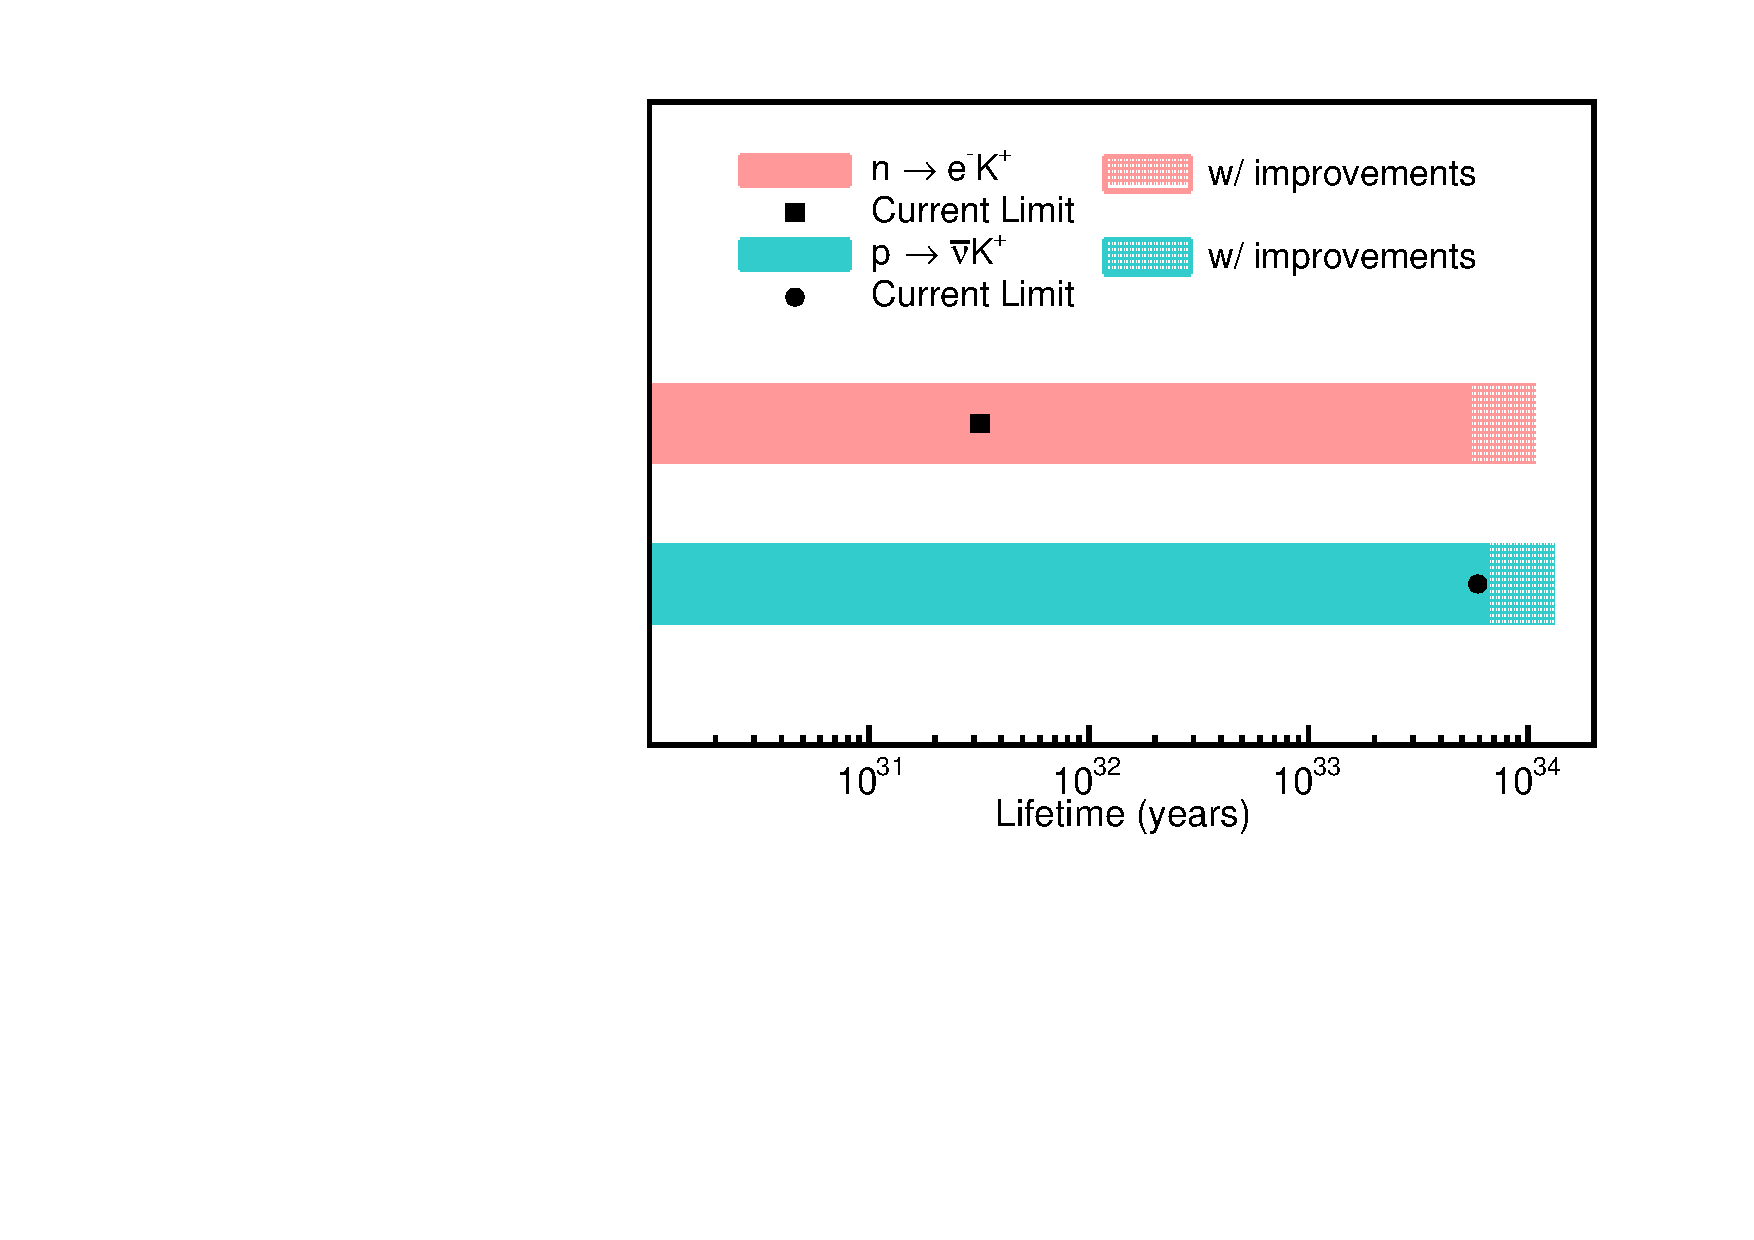
\includegraphics[width=0.8\textwidth]{sens.pdf}
%\end{dunefigure} 


%%%%%%%%%%%%%%%%%%%%%%%%%%%%%%%%%%%%%%%%%%%%%%%%%%%%%%%%%%%%%%%%
\section{Neutron-Antineutron Oscillations}
\label{sec:nonaccel-nnbar}

Neutron-antineutron (\nnbar) oscillation is a baryon number violating process that
has never been observed but is predicted by a number of \dword{bsm} theories~\cite{Phillips:2014fgb}. 
%In this context, baryon number conservation is an accidental
%symmetry rather than a fundamental one, which means baryon number violation
%does not stand against the fundamental gauge symmetries. 
Discovering baryon
number violation via observation of this process would have implications about the source of matter-antimatter
symmetry in our universe given Sakharov's conditions for such asymmetry to arise~\cite{Sakharov:1967dj}.
In particular, the neutron-antineutron oscillation (\nnbar) process violates
baryon number by two units and, therefore, could also have further implications for
the smallness of neutrino masses~\cite{Phillips:2014fgb}. 
Since the \nnbar transition operator is a six-quark operator, of Maxwellian dimension \num{9}, with a coefficient function of dimension (mass)$^{-5}$, while the proton decay operator is a four-fermion operator, of dimension \num{6}, with a coefficient function of dimension (mass)$^{-2}$, one might naively assume that \nnbar oscillations would always be suppressed relative
to proton decay as a manifestation of baryon number violation.  However, this is not necessarily the case; indeed, there are models~\cite{Nussinov:2001rb} in which proton decay is very strongly suppressed down to an unobservably small level, while \nnbar oscillations occur at a level comparable to present limits. This shows the
value of a search for \nnbar transitions at DUNE.
The \nnbar process is one of many possible baryon number violating processes that can be investigated in \dword{dune}. Searches for this process using
both free neutrons and nucleus-bound neutron states have continued 
since the 1980s. The current best \num{90}\% \dword{cl} limits on the (free) neutron oscillation lifetime are \SI{8.6e7}{\s} from free \nnbar searches and \SI{2.7e8}{\s} from nucleus-bound \nnbar searches~\cite{BaldoCeolin:1994jz,Abe:2011ky}.

Neutron-antineutron oscillations can be detected via the subsequent antineutron annihilation with a neutron or a proton. Table~\ref{tab:nnbar-br} shows the branching ratios for the antineutron annihilation modes applicable to intranuclear searches.  This annihilation event will have a distinct signature of a vertex with several emitted light hadrons, with total energy of twice the nucleon mass and zero net momentum. Reconstructing these hadrons correctly and measuring their energies is key to identifying the signal event. The main background for these \nnbar annihilation events is caused by atmospheric neutrinos. Most common among mis-classified events are \dword{nc} \dword{dis} events without a lepton in the final state. As with nucleon decay, nuclear effects and \dword{fsi} make the picture more complicated.


\begin{table}
\caption[\nnbar annihilation modes]{Effective branching ratios for antineutron annihilation in \argon40, as implemented
in GENIE.}
\begin{tabular}{p{.22\textwidth}p{.22\textwidth}p{.22\textwidth}p{.22\textwidth}}
\rowcolor{dunetablecolor} 
\multicolumn{2}{^c}{$\bar{n}+p$} & \multicolumn{2}{^c}{$\bar{n}+n$}\\
\rowcolor{dunetablecolor}
         Channel & Branching ratio & Channel & Branching ratio \\ \toprowrule
         $\pi^{+}\pi^{0}$ & 1.2\% & $\pi^{+}\pi^{-}$ & 2.0\% \\ \colhline
         $\pi^{+}2\pi^{0}$ & 9.5\% & $2\pi^{0}$ & 1.5\% \\ \colhline
         $\pi^{+}3\pi^{0}$ & 11.9\% & $\pi^{+}\pi^{-}\pi^{0}$ & 6.5\% \\ \colhline
         $2\pi^{+}\pi^{-}\pi^{0}$ & 26.2\% & $\pi^{+}\pi^{-}2\pi^{0}$ & 11.0\% \\ \colhline
         $2\pi^{+}\pi^{-}2\pi^{0}$ & 42.8\% & $\pi^{+}\pi^{-}3\pi^{0}$ & 28.0\% \\ \colhline
         $2\pi^{+}\pi^{-}2\omega$ & 0.003\% & $2\pi^{+}2\pi^{-}$ & 7.1\% \\ \colhline
         $3\pi^{+}2\pi^{-}\pi^{0}$ & 8.4\% & $2\pi^{+}2\pi^{-}\pi^{0}$ & 24.0\% \\ \colhline
          &  & $\pi^{+}\pi^{-}\omega$ & 10.0\% \\ \colhline
          &  & $2\pi^{+}2\pi^{-}2\pi^{0}$ & 10.0\% \\ \colhline
\label{tab:nnbar-br}
\end{tabular}
\end{table}

\subsection{Sensitivity to Intranuclear Neutron-Antineutron Oscillations in DUNE}
\label{subsec:nonaccel-nnbar-dunesensitivity}

The simulation of neutron-antineutron oscillation was developed~\cite{Hewes:2017xtr} and implemented in \dword{genie}. This analysis uses \dword{genie} v.2.12.10.
%(see Table~\ref{tab:genie-antineutron} in Appendix~\ref{sec:tools-app-generator} for a list of interaction channels available in \dword{genie}).  
Implementing this process in \dword{genie} used \dword{genie}'s existing modeling of Fermi momentum and binding energy for both the oscillating neutron and the nucleon with which the resulting antineutron annihilates.   Once a neutron has oscillated to an antineutron in a nucleus, the antineutron has a $18/39$ chance of annihilating with a proton in argon, and a $21/39$ chance of annihilating with a neutron. The energies and momenta of the annihilation products are assigned randomly but consistently with four-momentum conservation. The products of the annihilation process follow the branching fractions (shown in Table~\ref{tab:nnbar-br}) measured in low-energy antiproton annihilation on hydrogen.
Since the annihilation products are produced inside the nucleus, \dword{genie} further models re-interactions of those products as they propagate in the nucleus (until they escape the nucleus).  The \dword{fsi} are simulated using the $hA2015$ model in \dword{genie} as described in Section~\ref{sec:final-state-interactions}.

Figure~\ref{fig:pi_FSI_m} shows the momentum distributions for charged and neutral pions before \dword{fsi} and after \dword{fsi}. These distributions show the \dword{fsi} makes both charged and neutral pions less energetic.  The effect of \dword{fsi} on pion multiplicity is also rather significant; \num{0.9}\% of the events have no charged pions before \dword{fsi}, whereas after \dword{fsi} \num{11.1}\% of the events have no charged pions. In the case of the neutral pion, \num{11.0}\% of the events have no neutral pions before \dword{fsi}, whereas after \dword{fsi}, \num{23.4}\% of the events have no neutral pions. The decrease in pion multiplicity is primarily due to pion absorption in the nucleus. Another effect of \dword{fsi} is nucleon knockout from pion elastic scattering. Of the events, \num{94}\% have at least one proton from \dword{fsi} and \num{95}\% of the events have at least one neutron from \dword{fsi}. Although the kinetic energy for these nucleons peak at a few tens of \si{\MeV}, the kinetic energy can be as large as hundreds of \si{\MeV}.  In summary, the effects of \dword{fsi} in \nnbar become relevant because they modify the kinematics and topology of the event. For instance, even though the decay modes of Table \ref{tab:nnbar-br} do not include nucleons in their decay products, nucleons appear with high probability after \dword{fsi}.

\begin{dunefigure}
[Final state interactions in \nnbar]{fig:pi_FSI_m}
{Momentum of an individual charged pion before and after final state interactions (left): momentum of an individual neutral pion before and after final state interactions (right).}
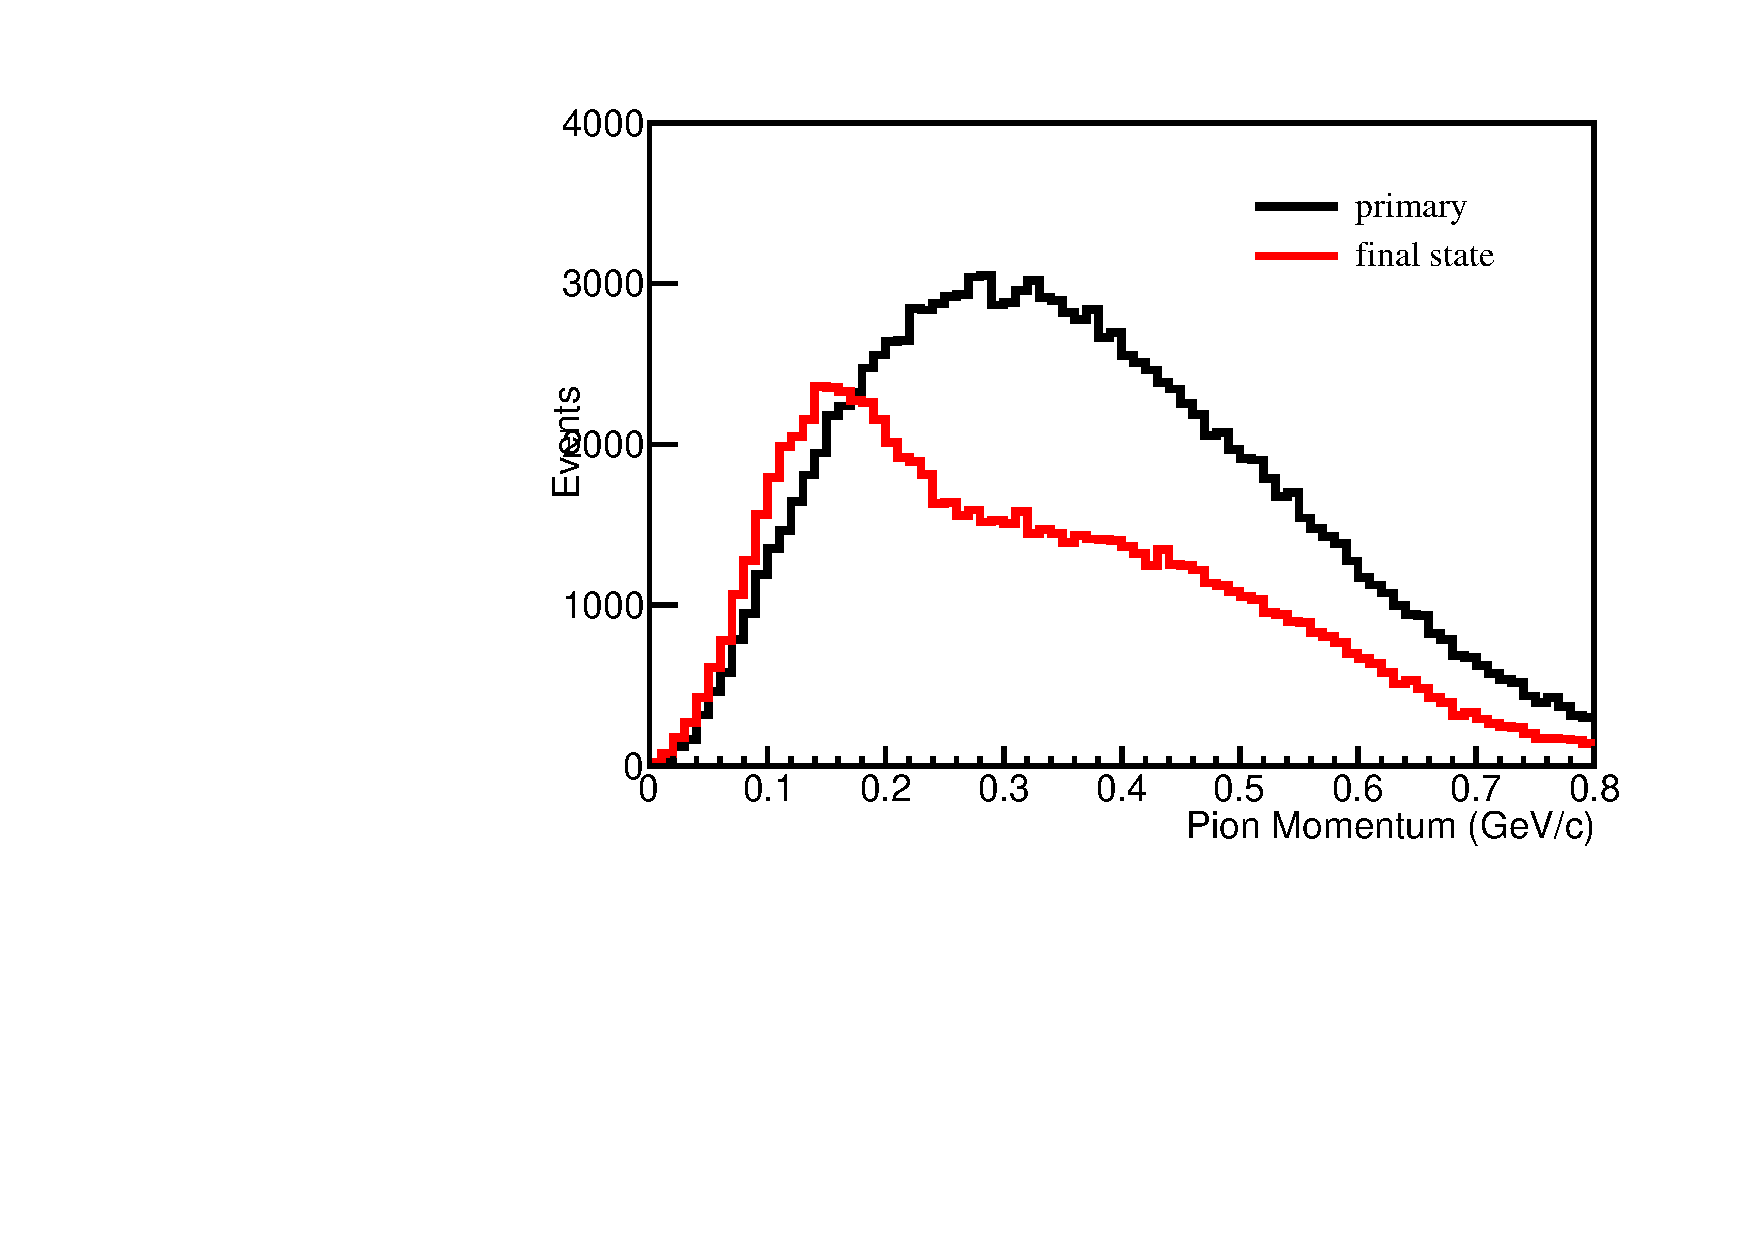
\includegraphics[width=0.49\textwidth]{pi_mom.pdf}
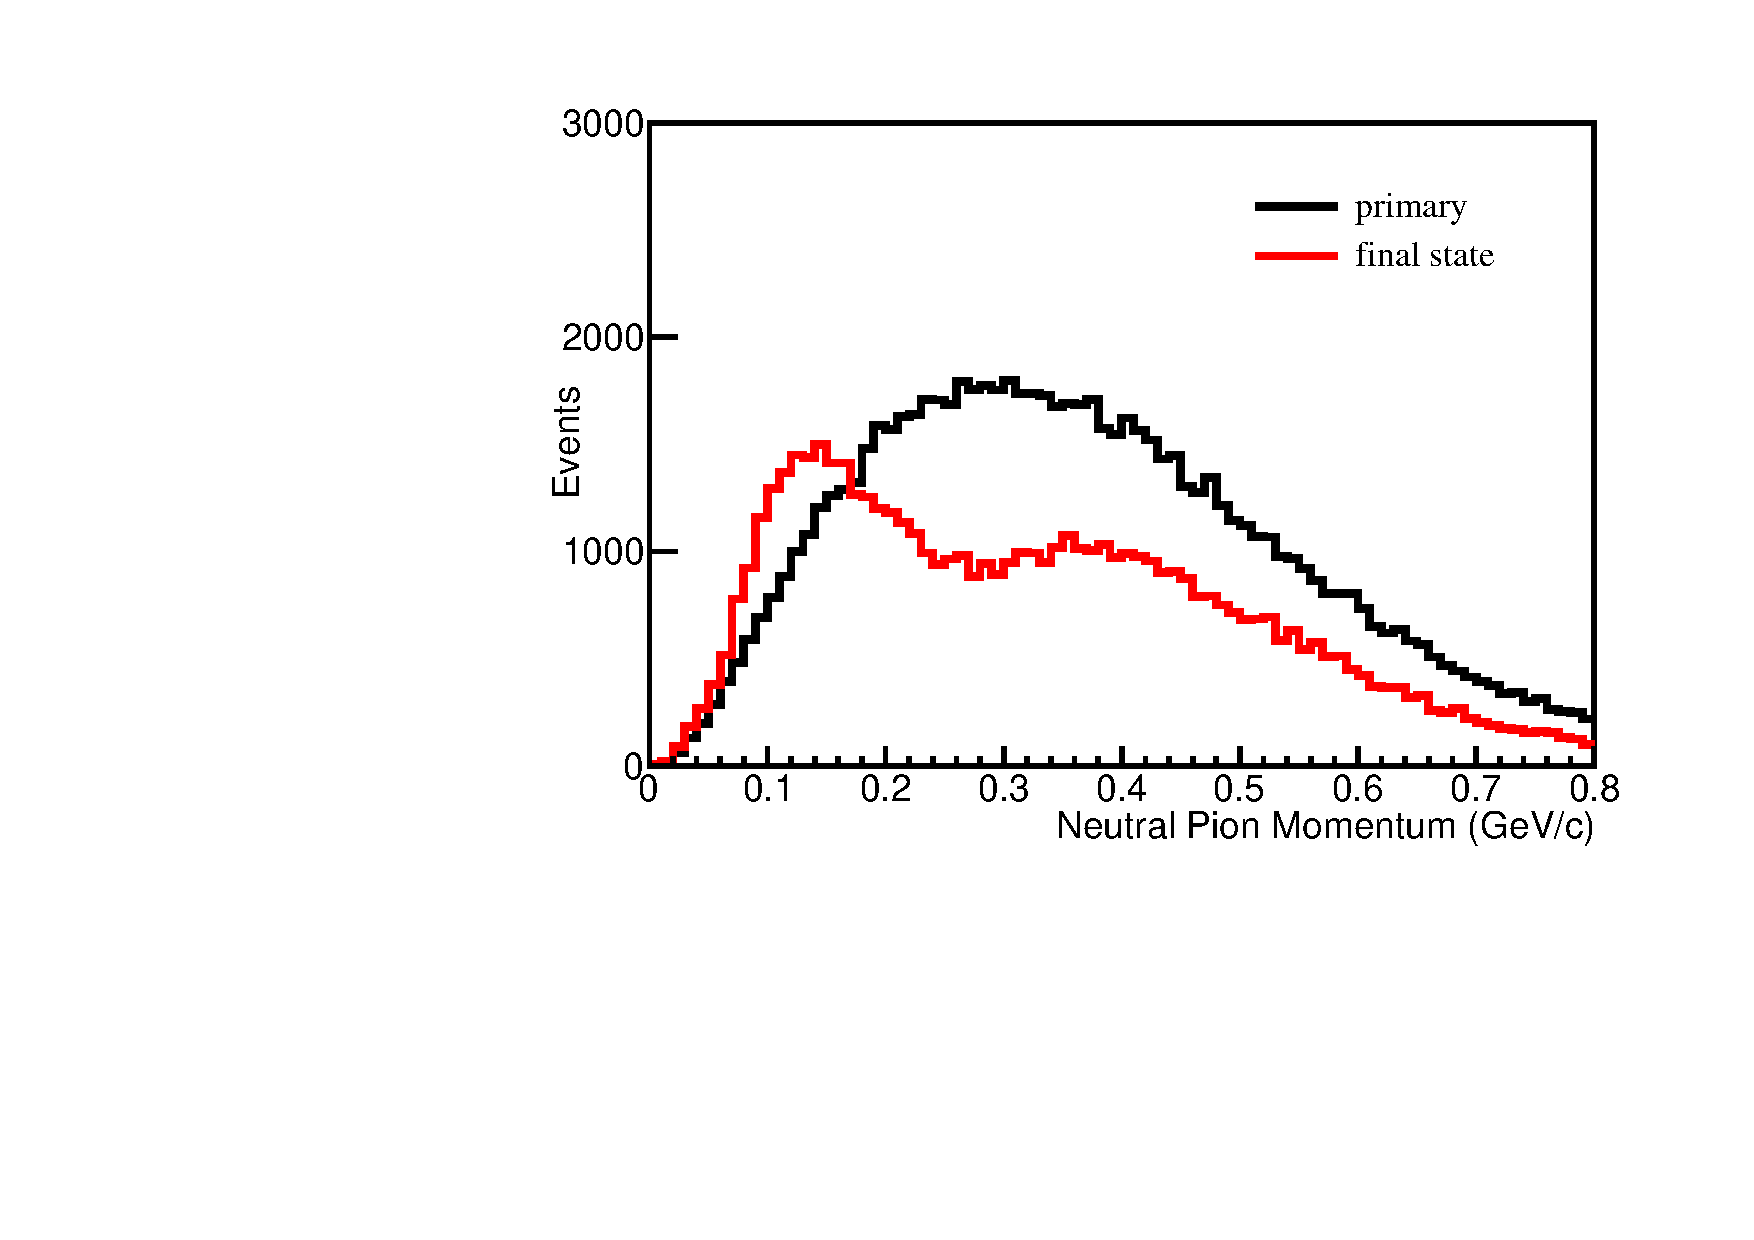
\includegraphics[width=0.49\textwidth]{pizero_mom.pdf}
\end{dunefigure} 

The main background process in search of bound \nnbar oscillation in \dword{dune} is assumed to be atmospheric neutrino interactions in the detector.  This is simulated in \dword{genie} as described in Section~\ref{sec:ndkbkgd}.

As with the \ptoknubar analysis, two distinct methods of reconstruction and event selection have been applied in this search. One involves traditional reconstruction methods (\threed track and vertex reconstruction by \dword{pma}); the other involves image classification 
of \twod images of reconstructed hits (\dword{cnn}). The two methods, combined in the form of a multivariate analysis, uses the image classification score with other physical observables extracted from traditional reconstruction.  A \dword{bdt} classifier is used. Ten variables are used in the \dword{bdt} event selection, including number of reconstructed tracks and showers; variables related to visible energy deposition; $PIDA$ and $dE/dx$; reconstructed momentum; and CNN score.  Figure~\ref{fig:bdt_nnbar} shows the distribution of the \dword{bdt} output for signal and background.

\begin{dunefigure}
[\nnbar Boosted Decision Tree response]{fig:bdt_nnbar}
{Boosted Decision Tree response for \nnbar oscillation for signal (blue) and background (red).}
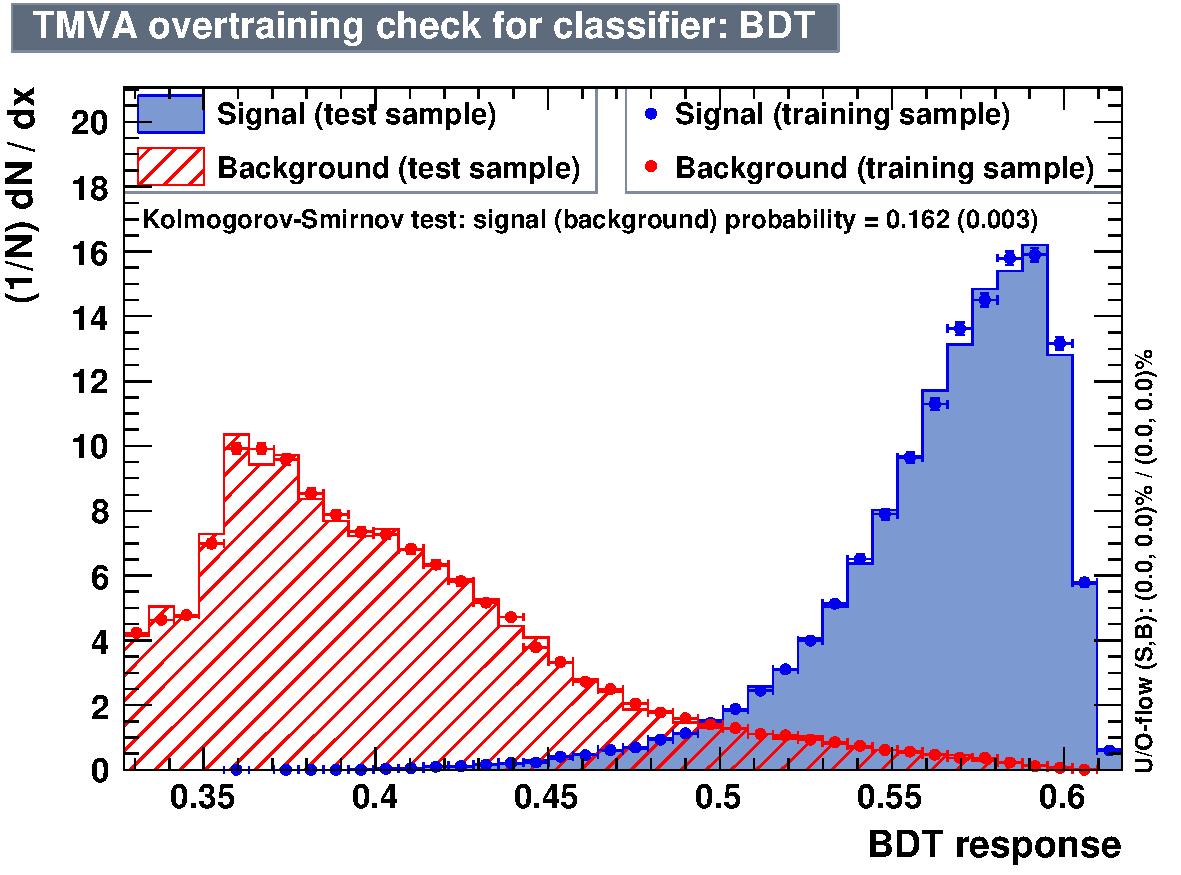
\includegraphics[width=0.8\textwidth]{BDT_nnbar.pdf}
\end{dunefigure} 

Figure~\ref{fig:nnbar_sig} shows an \nnbar event with high \dword{bdt} response value (\num{0.592}). Showers from neutral pions are shown in red, blue, yellow, and green. The reconstructed charged pion tracks are shown as dark green and maroon lines. The topology of this event is consistent with charged pion and neutral pion production. 

The left side plot in Figure~\ref{fig:nnbar_bkgd} shows a \dword{nc} atmospheric neutrino interaction $\nu_{e}+n\rightarrow \nu_{e}+p+p$ with a low \dword{bdt} response value (\num{0.388}). This type of interaction is easily distinguished from the signal.  The two protons from the \dword{nc} interaction are reconstructed as tracks, and no shower activity is present. However, the right side plot in Figure~\ref{fig:nnbar_bkgd} displays a \dword{cc} atmospheric neutrino interaction $\nu_{e}+n\rightarrow {e}^{-}+p+\pi +p$ with a high \dword{bdt} response value (\num{0.598}). This background event mimics the signal topology by having multi-particle production and an electromagnetic shower. Further improvements in shower reconstruction, especially $dE/dx$, should help in classifying these types of background events in the future because the electron shower $dE/dx$ differs from the $dE/dx$ of a shower induced by a gamma-ray.

\begin{dunefigure}
[Event display for well-classified \nnbar signal event]{fig:nnbar_sig}
{Event display for a well-classified \nnbar signal event.  The vertical axis is time ticks (each time tick corresponds to \SI{500}{\ns}), and the horizontal axis is wire number.  The bottom view is induction plane one, middle is induction plane two, and the top is the collection plane.  The color represents the charge deposited in each hit.}
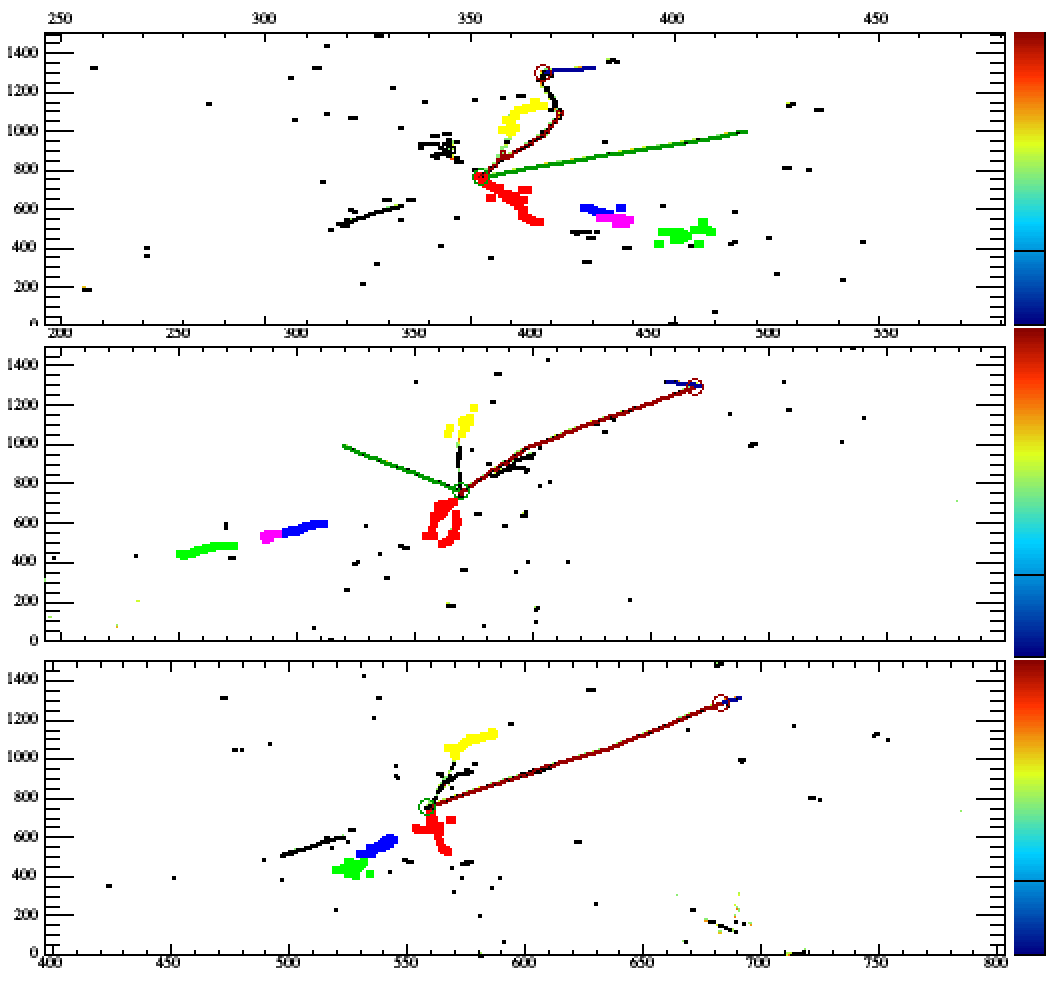
\includegraphics[width=0.8\textwidth]{nnbar_sig.png}
\end{dunefigure} 

\begin{dunefigure}
[Event displays for \nnbar background events]{fig:nnbar_bkgd}
{Event displays for \nnbar backgrounds.  The vertical axis is time ticks (each time tick corresponds to \SI{500}{\ns}), and the horizontal axis is wire number.  The bottom view is induction plane one, middle is induction plane two, and the top is the collection plane.  The color represents the charge deposited in each hit.  The left plot shows an atmospheric neutrino interaction unlikely to be classified as signal. The right plot shows an atmospheric neutrino interaction which could make it into the selected sample.}
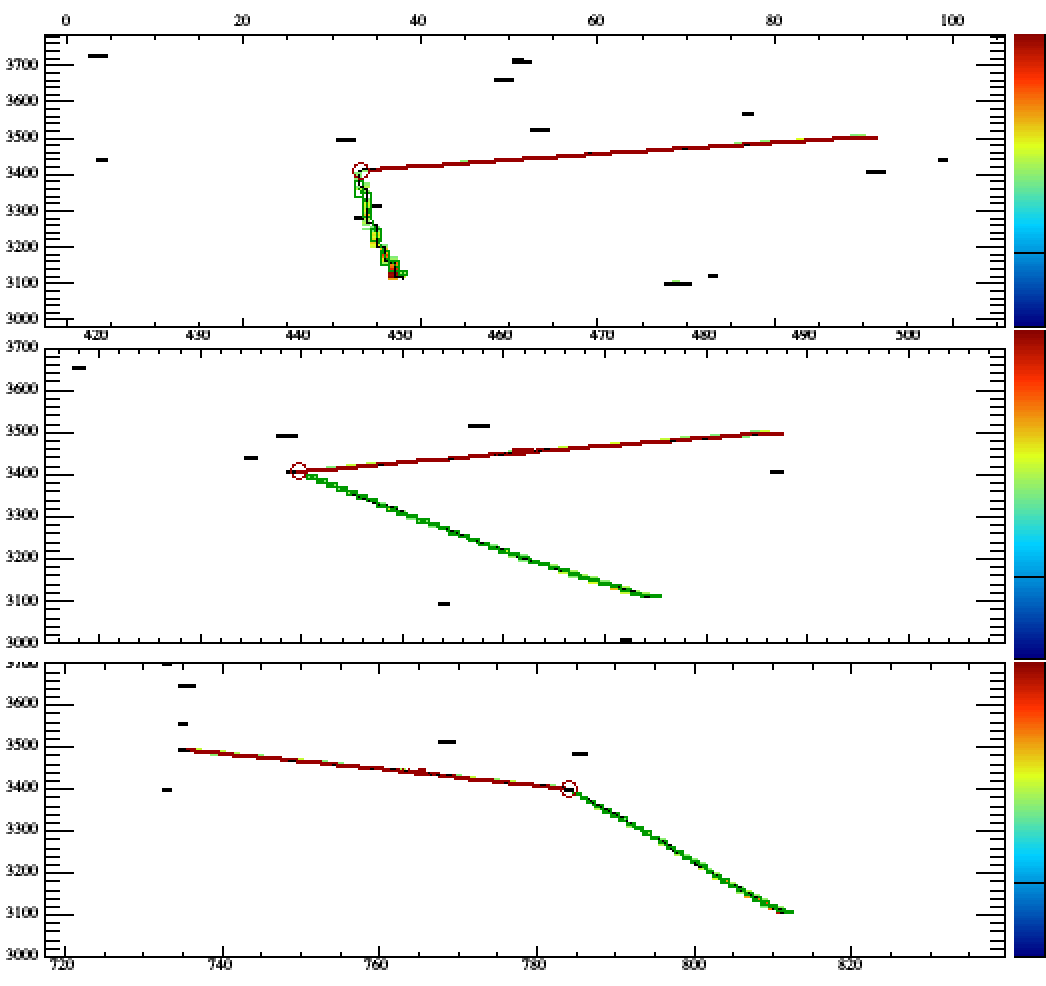
\includegraphics[width=0.49\textwidth]{nnbar_bkgd_ev2.png}
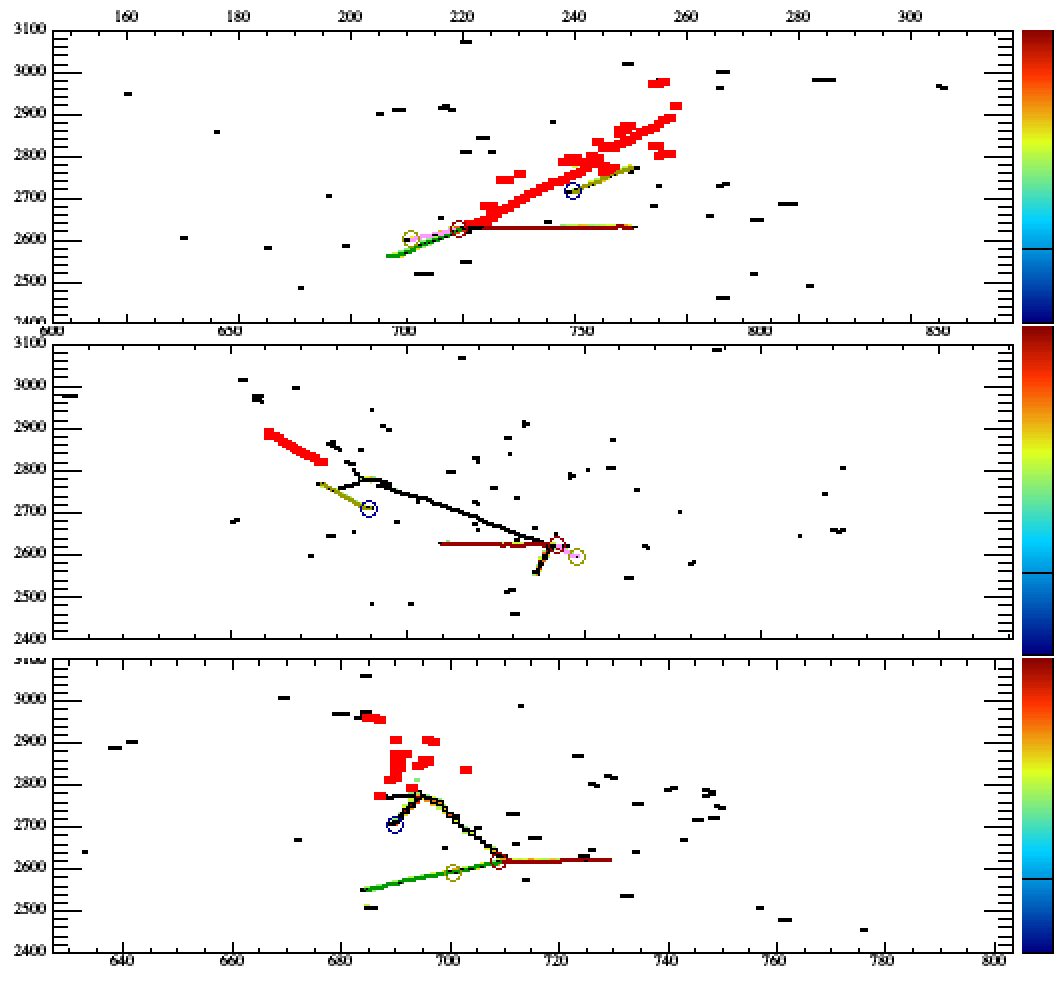
\includegraphics[width=0.49\textwidth]{nnbar_bkgd_ev1.png}
\end{dunefigure} 

The sensitivity to the \nnbar oscillation lifetime can be calculated for a given exposure, the efficiency of selecting signal events, and the background rate along their uncertainties. The lifetime sensitivity is obtained at \num{90}\% \dword{cl} for the bound neutron. Then, the lifetime sensitivity for a free neutron is acquired using the conversion from nucleus bounded neutron to free neutron \nnbar oscillation~\cite{Friedman:2008es}.  
%As a first estimate of systematic uncertainties, the uncertainties from the \nnbar oscillation search by the \superk collaboration~\cite{Abe:2011ky} are used in this analysis.  While the detailed breakdown of the uncertainties in \dword{dune} will likely be very different, the overall size of the uncertainties (\num{3}\% on exposure, \num{25}\% on signal efficiency, and \num{25}\% on background rejection) are expected to be roughly similar.  Studies to evaluate these uncertainties in \dword{dune} are in progress.
The uncertainties on the signal efficiency and background rejection are conservatively estimated to be \num{25}\%.  A detailed evaluation of the uncertainties is in progress.

The free \nnbar oscillation lifetime, $\tau_{n-\bar{n}}$, and bounded \nnbar oscillation lifetime, $T_{n-\bar{n}}$, are related to each other through the suppression factor $R$ as
%
\begin{equation}
    \tau^{2}_{n-\bar{n}} = \frac{T_{n-\bar{n}}}{R} ~.
    \label{eq:tau}
\end{equation}
The suppression factor $R$ varies for different nuclei. This suppression factor was calculated for $^{16}$O and $^{56}$Fe~\cite{Friedman:2008es}. The $R$ for $^{56}$Fe, \SI{0.666e23}{\per\s}, is used in this analysis for \argon40 nuclei.

The best bound neutron lifetime limit is achieved using a signal efficiency of \num{8.0}\% at the background rejection probability of \num{99.98}\%. The \num{90}\% \dword{cl} limit of a bound neutron lifetime is \SI{6.45e32}{years} for a \SI{400}{\ktyr} exposure. The corresponding limit for the oscillation time of free neutrons is calculated to be \SI{5.53e8}{\s}. This is approximately an improvement by a factor of two from the current best limit, which comes from \superk~\cite{Abe:2011ky}.  Planned improvements to this analysis include improved \dword{cnn} performance and better estimates of systematic uncertainties.  As with nucleon decay, searches for \nnbar oscillations performed by \dword{dune} and those performed by \superk or \hyperk are highly complementary.  Should a signal be observed in any one experiment, confirmation from another experiment with a different detector technology and backgrounds would be very powerful. 

%%%%%%%%%%%%%%%%%%%%%%%%%%%%%%%%%%%%%%%%%%%%%%%%%%%%%%%%%%%%%%%%
\section{Physics with Atmospheric Neutrinos}
\label{sec:nonaccel-atm}

Atmospheric neutrinos are a unique tool for studying neutrino oscillations: the oscillated flux contains all flavors of neutrinos and antineutrinos, is very sensitive to matter effects and to both \dm{} parameters, and covers a wide range of $L/E$. In principle, all oscillation parameters could be measured, with high
complementarity to measurements performed with a neutrino beam. In addition, atmospheric neutrinos are available all the time, in particular before the beam becomes operational. The \dword{dune} \dword{fd}, with its large mass and the overburden to protect it from atmospheric muon background, is an ideal tool for these studies.  Given the strong overlap in event topology and energy scale with beam neutrino interactions, most requirements will necessarily be met by the \dword{fd} design. Additional requirements include a self-trigger because atmospheric neutrino events are asynchronous with accelerator timing and a more stringent demand on neutrino direction reconstruction.

\subsection{Oscillation Physics with Atmospheric Neutrinos}
\label{sec:nonaccel-atm-oscillations}

Sensitivity to oscillation parameters with atmospheric neutrinos in \dword{dune} has been evaluated.
%with a 
%dedicated simulation, reconstruction and analysis chain. 
The fluxes of each neutrino species were computed at the \dword{fd} location after 
oscillation. Interactions in the \dword{lar} medium were simulated with the \dword{genie} event 
generator. Detection thresholds and energy resolutions based on full 
simulations were applied to the outgoing particles to take 
detector effects into account. Events were classified as fully contained or partly contained by placing the vertex at a random position inside the 
detector and tracking the lepton until it reaches the edge of the detector.
Partly contained events 
are those where a final state muon exits the detector.  The number of events expected 
for each flavor and category is summarized in Table~\ref{tab:atmos_rates}.

\begin{dunetable}
[Atmospheric neutrino event rates per year in different analysis categories]
{lc}
{tab:atmos_rates}
{Atmospheric neutrino event rates per year in \SI{40}{\kt} of fiducial mass including oscillations in different analysis categories}
Sample   &  Event rate per year \\ \toprowrule
fully contained electron-like   & \num{1600} \\ \colhline
fully contained muon-like       & \num{2400} \\ \colhline
partly contained muon-like   & \num{790} \\ 
\end{dunetable}

Figure~\ref{fig:lovere} shows the expected $L/E$ distribution for high-resolution, muon-like 
events from a \SI{400}{\ktyr} exposure. The data provide excellent resolution of the 
first two oscillation nodes, even with the expected statistical uncertainty.
In performing oscillation fits, the data in each flavor/containment category are 
binned in energy and zenith angle.

\begin{dunefigure}
[Reconstructed $L/E$ Distribution of `High-Resolution' Atmospheric Neutrinos]{fig:lovere}
{Reconstructed $L/E$ Distribution of `High-Resolution'
$\mu$-like atmospheric neutrino events in a \SI{400}{\ktyr} exposure with and
without oscillations (left), and the ratio of the two (right), with the error bars indicating the size of the statistical uncertainty.}
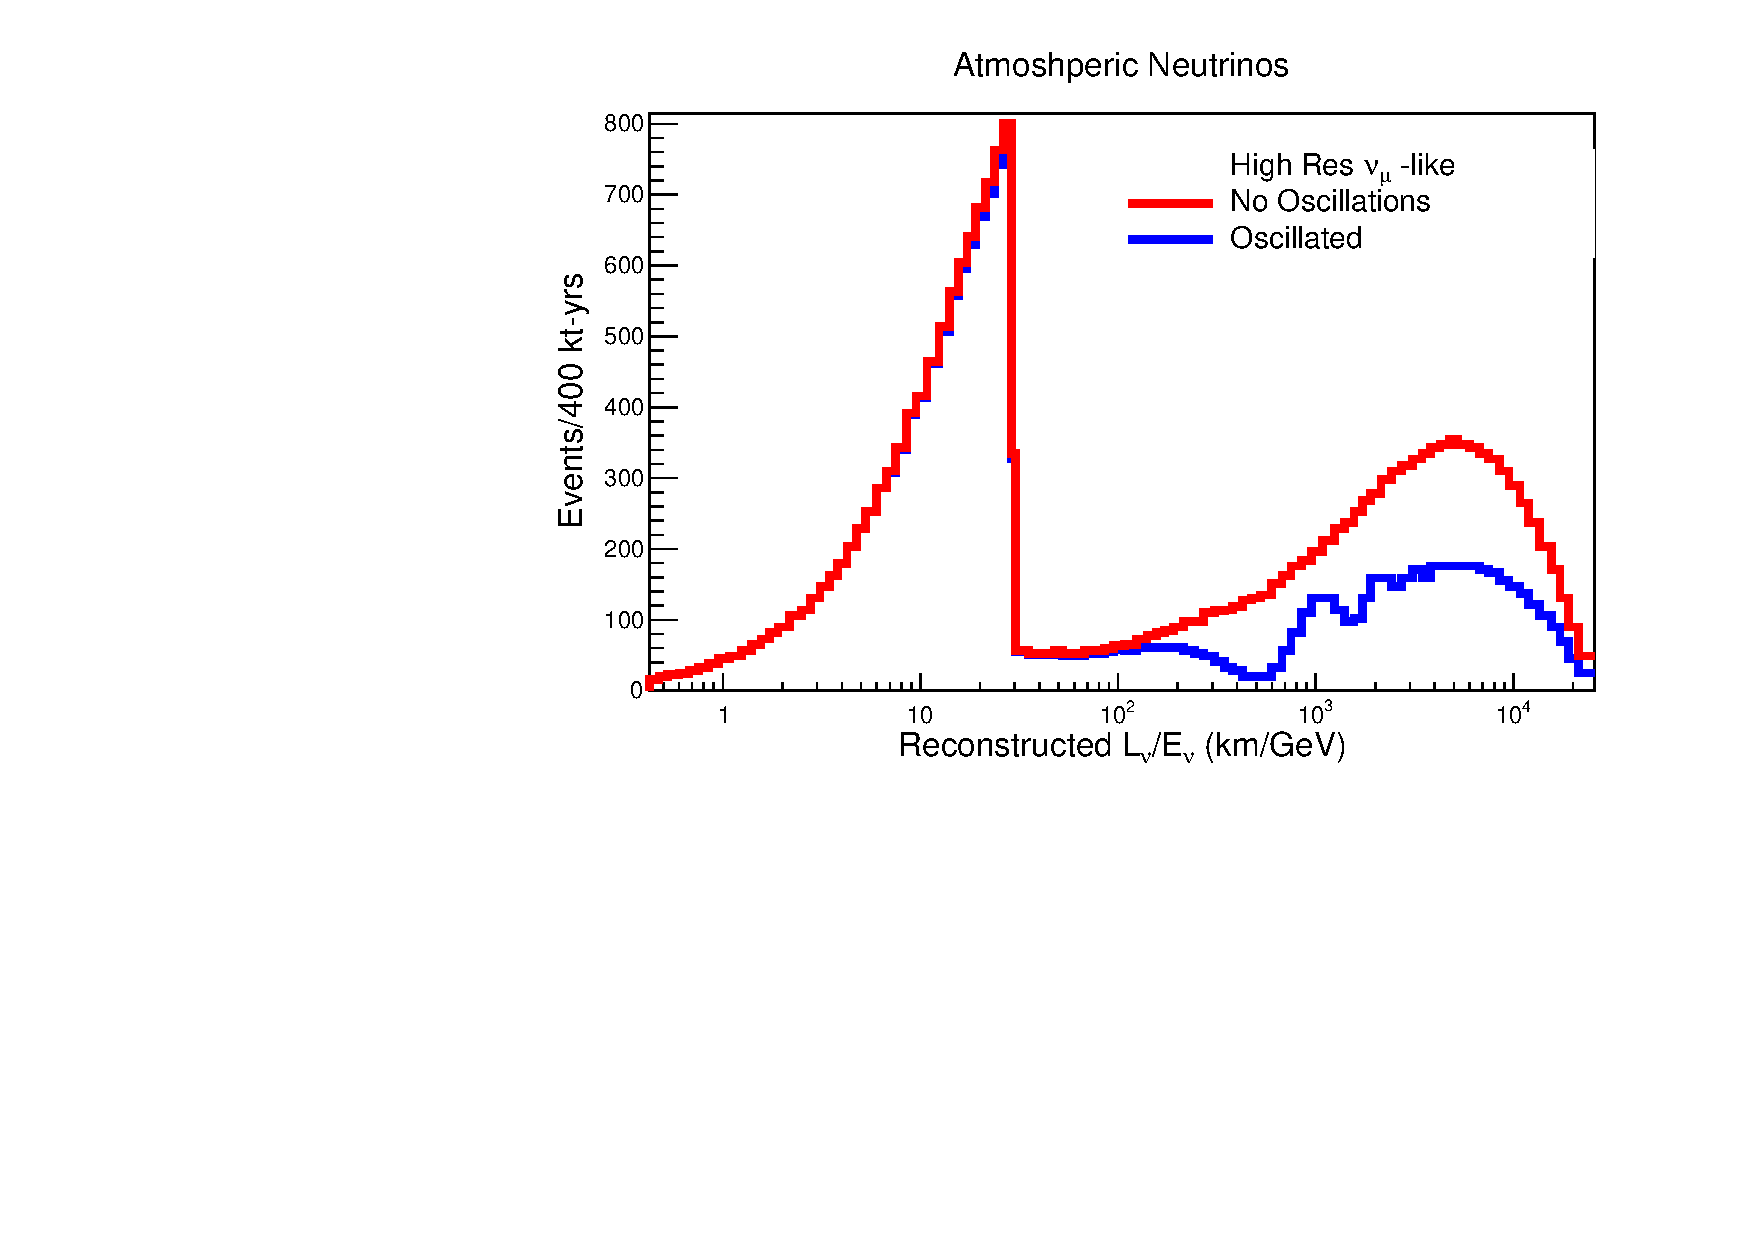
\includegraphics[width=0.49\textwidth]{atm_spectrum_LoverE_400.pdf}
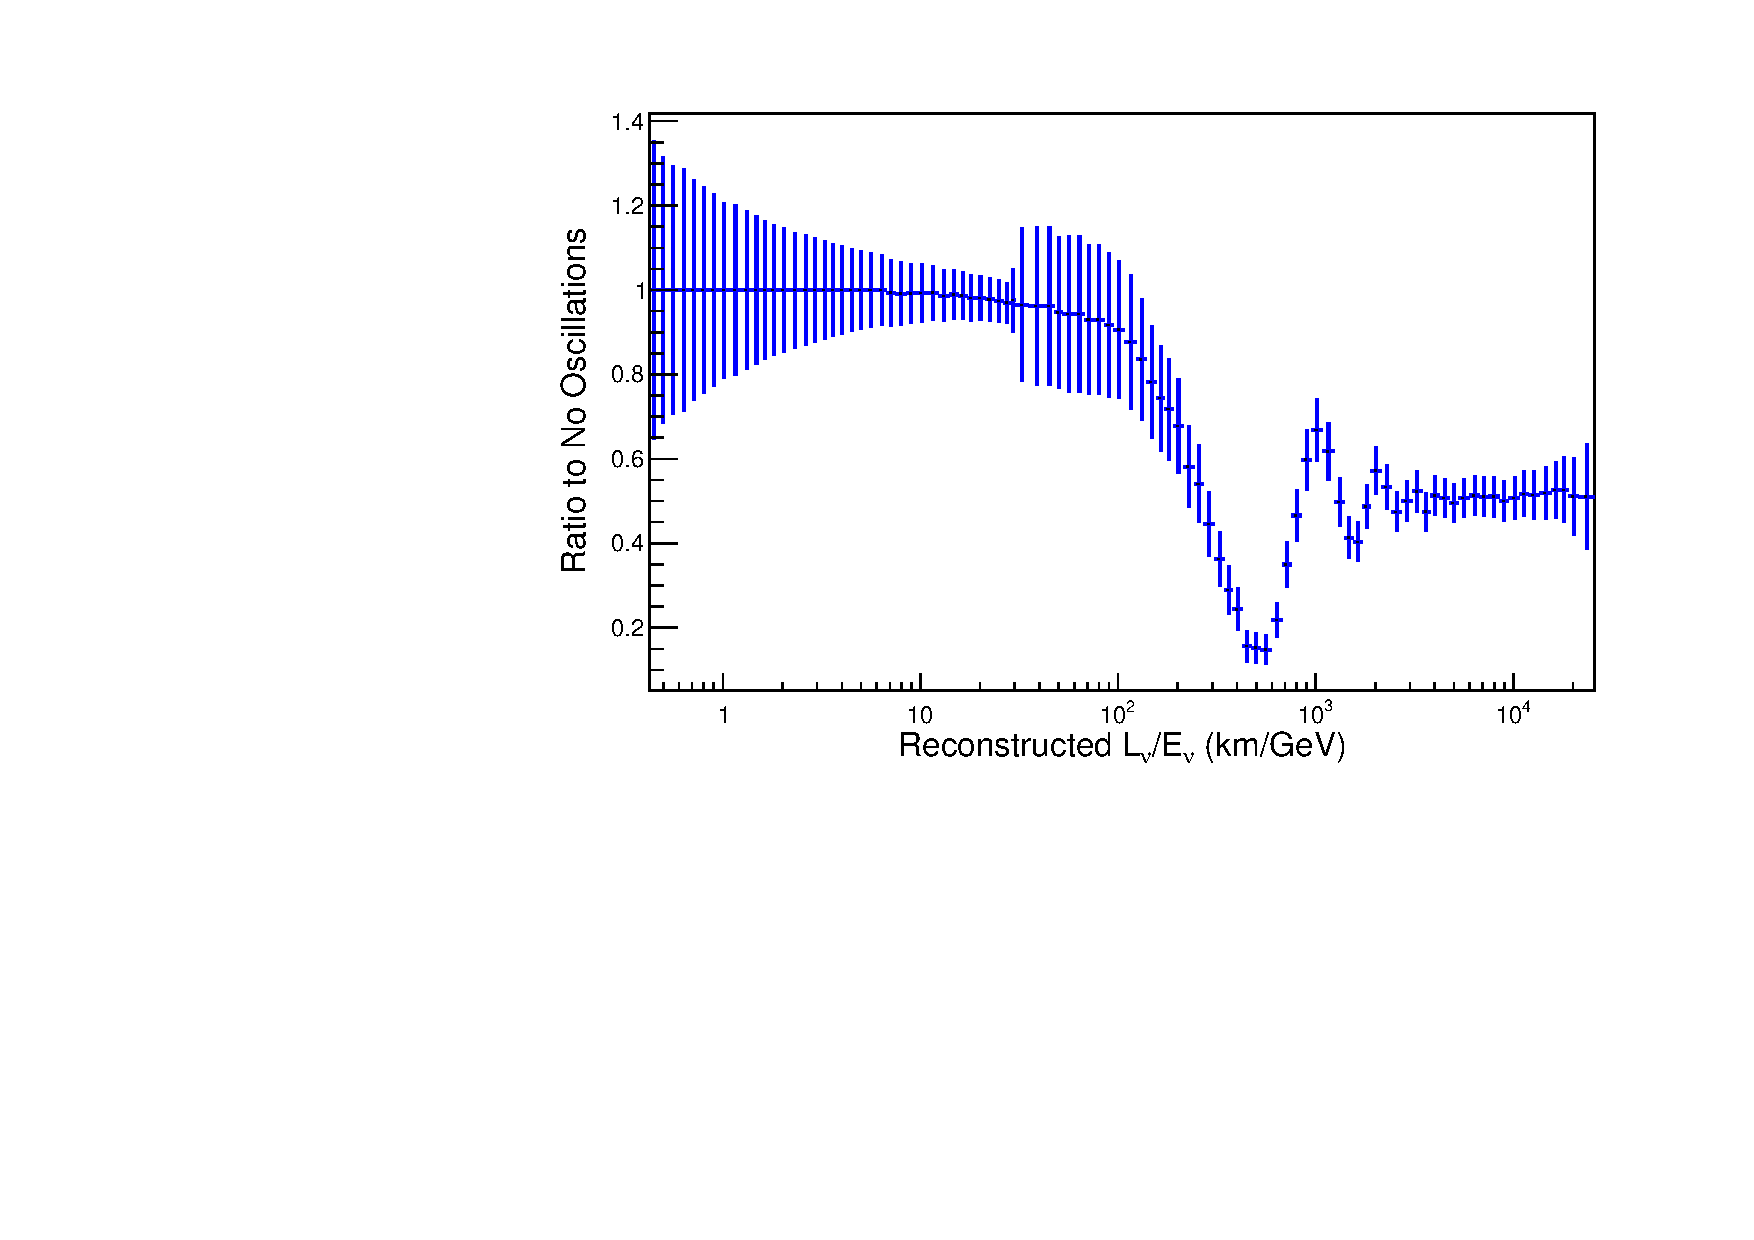
\includegraphics[width=0.49\textwidth]{atm_spectrum_LoverE_400_2.pdf}
\end{dunefigure}

When neutrinos travel through the Earth, the \dword{msw} resonance influences 
electron neutrinos in the few-\si{GeV} energy range. More precisely, the resonance 
occurs for \nue in the case of normal ordering and for \anue in the case of inverted ordering.

The mass ordering sensitivity can be greatly enhanced if neutrino and antineutrino events can be 
separated. The \dword{dune} \dword{fd} will not be magnetized, but its high-resolution 
imaging offers possibilities for tagging features of events that provide statistical 
discrimination between neutrinos and antineutrinos. For the sensitivity calculations, 
two such tags were included: a proton tag and a decay electron tag. 

Figure~\ref{fig:atm_mh} shows the mass ordering sensitivity as a function of the fiducial exposure.  Over this range of fiducial exposures, the sensitivity essentially follows the square root of the exposure, indicating that the measurement is not systematics-limited. Unlike beam measurements, the sensitivity to the mass ordering with atmospheric neutrinos is nearly independent of the \dword{cp} violating phase.  The sensitivity comes from both electron neutrino appearance as well as muon neutrino disappearance and depends strongly on the true value of \sinst{23}, as shown in Figure~\ref{fig:atm_mh}. For comparison, the sensitivity for \hyperk atmospheric neutrinos with a \SI{1900}{\ktyr} exposure is also shown.

\begin{dunefigure}
[Mass Ordering Sensitivity vs. Exposure for Atmospheric Neutrinos]{fig:atm_mh}
{Sensitivity to mass ordering using atmospheric neutrinos as a function of fiducial exposure in \dword{dune} (left) and as a function of the true value of \sinst{23} (right).  For comparison, \hyperk sensitivities are also shown \cite{Abe:2018uyc}.}
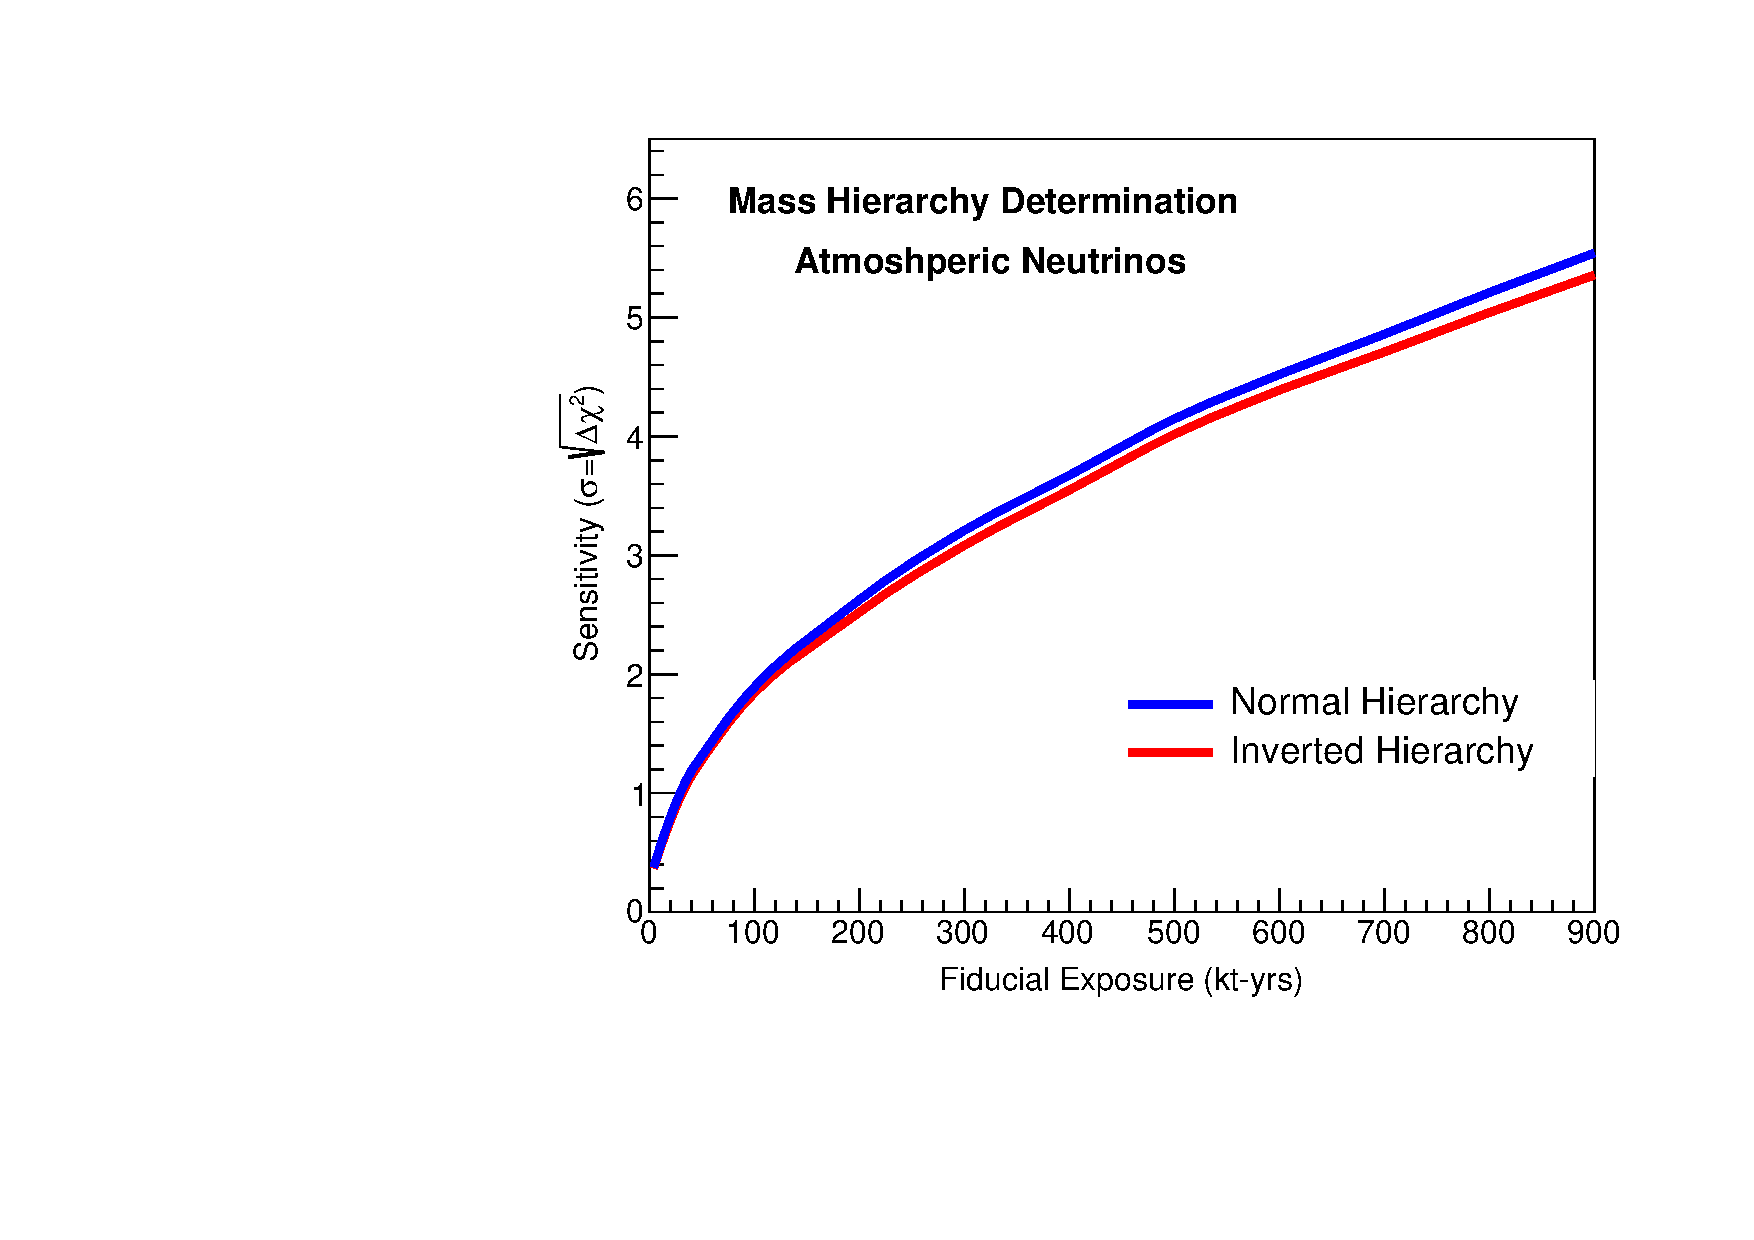
\includegraphics[width=0.41\textwidth]{atm_mh_vs_exposure.pdf}
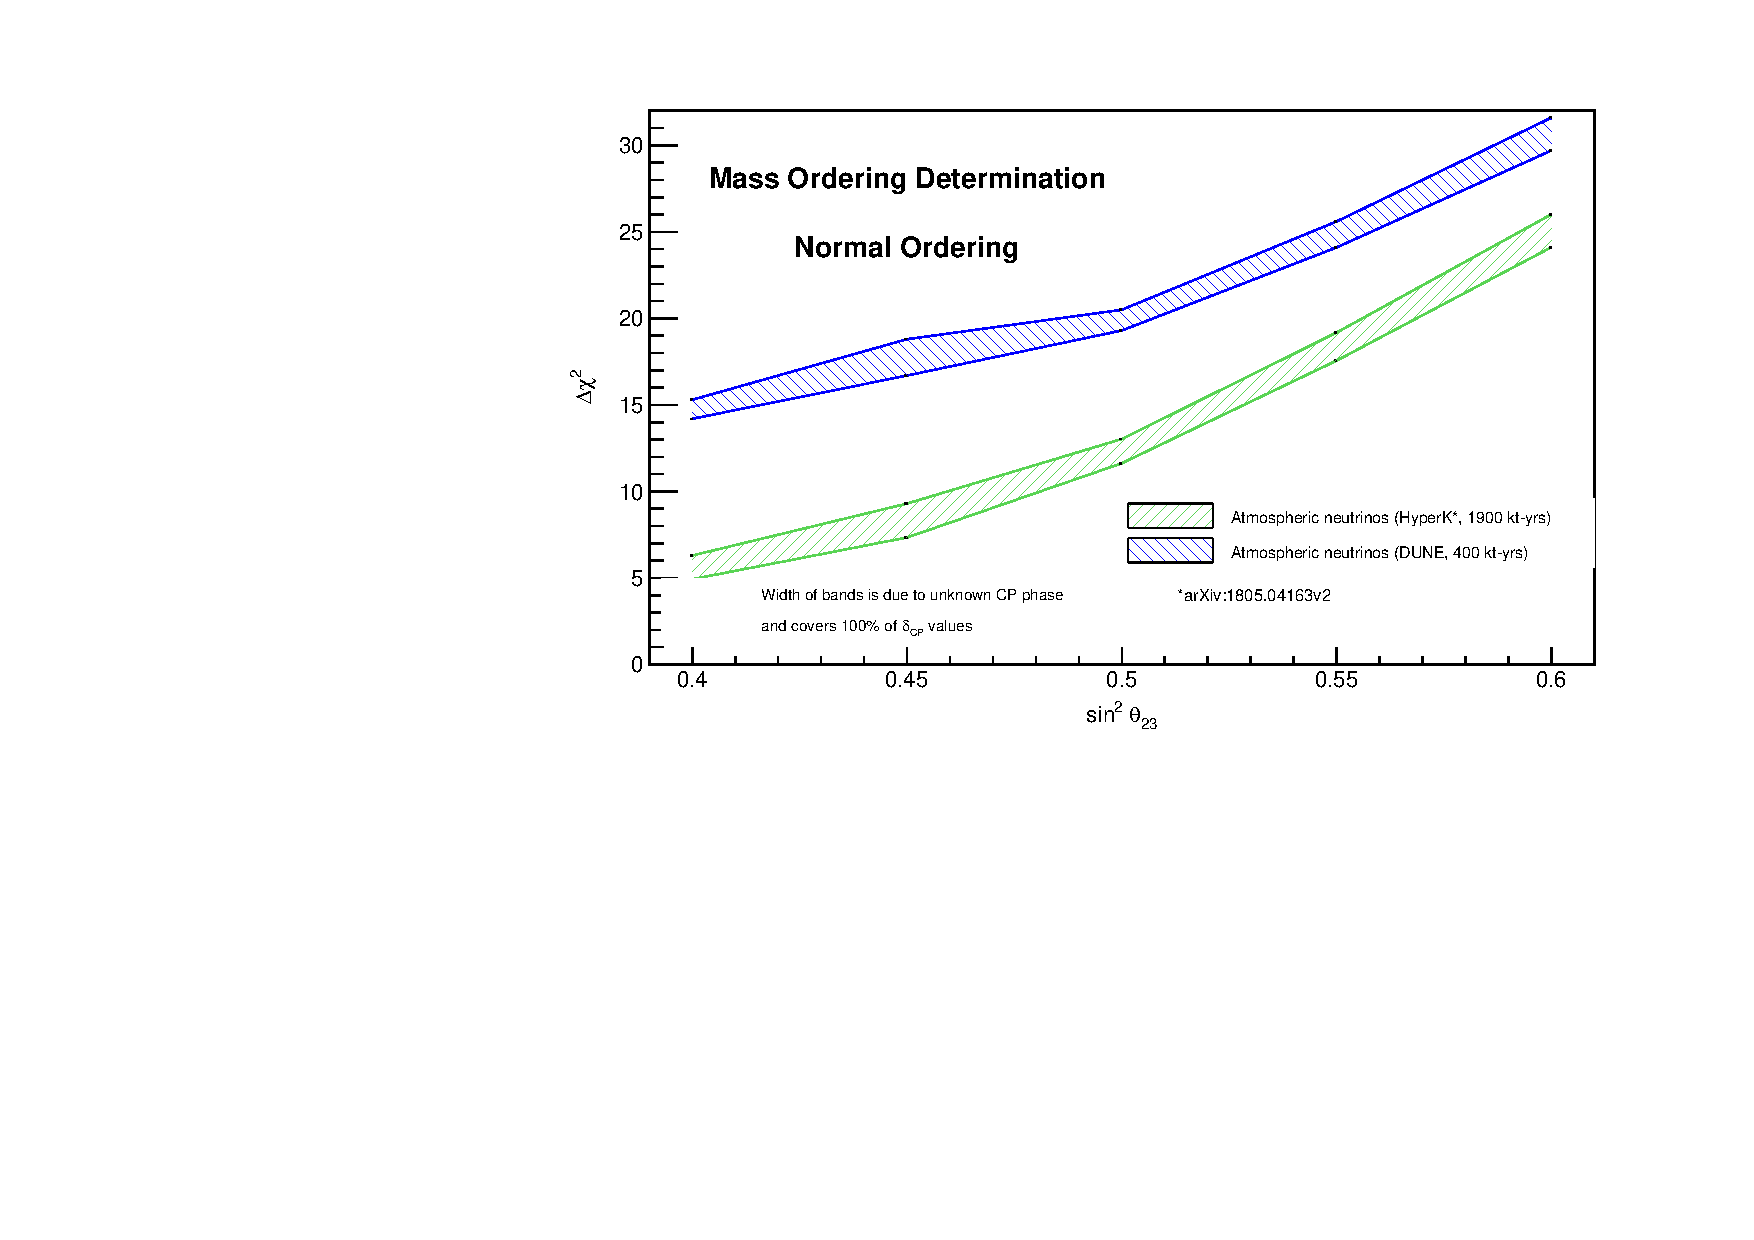
\includegraphics[width=0.58\textwidth]{MHS_DUNEvsHK.pdf}
\end{dunefigure}

In the two-flavor approximation, neutrino oscillation probabilities depend on 
\sinst, which is invariant when changing $\theta$ to $\pi/2-\theta$. In this case, the octant degeneracy remains for $\theta_{23}$ in the leading order terms of the full 
three-flavor oscillation probability, making it impossible to determine whether $\theta_{23}< \pi/4$ or 
$\theta_{23}> \pi/4$. Accessing full three-flavor oscillation with atmospheric neutrinos 
should help solve the ambiguity.


These analyses will provide an approach complementary to the beam neutrino approach. For instance, atmospheric neutrinos should resolve  degeneracies present in beam analyses because the mass ordering sensitivity is essentially independent of \deltacp. Atmospheric neutrino data will be acquired 
even in the absence of the beam and will provide a useful sample for developing reconstruction software, analysis methodologies, and calibrations.  Atmospheric neutrinos provide a window into a range of new physics scenarios, and may allow \dword{dune} to place limits on Lorentz and \dword{cpt} violation (see Section~\ref{sec:nonaccel-atm-bsm}), 
non-standard interactions~\cite{Chatterjee:2014gxa}, mass-varying neutrinos~\cite{Abe:2008zza}, and
sterile neutrinos~\cite{Abe:2014gda}.
Recent studies have also indicated that sub-GeV atmospheric neutrinos could be used to exclude some values of \deltacp independently from the beam neutrino measurements~\cite{Kelly:2019itm}.

\subsection{BSM Physics with Atmospheric Neutrinos}
\label{sec:nonaccel-atm-bsm}

Studying \dword{dune} atmospheric neutrinos is a promising approach
to search for \dword{bsm} effects such as Lorentz and \dword{cpt} violation,
which has been hypothesized
to emerge from an underlying Planck-scale theory like strings~\cite{Kostelecky:1988zi,Kostelecky:1991ak}.
The comprehensive realistic effective field theory
for Lorentz and \dword{cpt} violation,
the \dword{sme}~\cite{Kostelecky:1994rn,Colladay:1996iz,Colladay:1998fq,Kostelecky:2003fs},
is a powerful and calculable framework
for analyzing experimental data.
All \dword{sme} coefficients for Lorentz and \dword{cpt} violation
governing the propagation and oscillation of neutrinos
have been enumerated~\cite{Kostelecky:2003cr,Kostelecky:2011gq},
and many experimental measurements of \dword{sme} coefficients 
have been performed to date~\cite{Kostelecky:2008ts}.
Nonetheless,
much of the available \dword{sme} coefficient space 
in the neutrino sector remains unexplored.

Experimental signals predicted by the \dword{sme} include
corrections to standard neutrino-neutrino 
and antineutrino-antineutrino mixing probabilities,
oscillations between neutrinos and antineutrinos,
and modifications of oscillation-free propagation,
all of which incorporate unconventional dependencies
on the magnitudes and directions of momenta and spin.
For \dword{dune} atmospheric neutrinos,
the long available baselines,
the comparatively high energies accessible,
and the broad range of momentum directions
offer advantages that can make possible great
improvements 
in sensitivities to certain types of Lorentz and \dword{cpt} violation~\cite{Kostelecky:2003cr,Kostelecky:2011gq,Kostelecky:2003xn,Kostelecky:2004hg,Diaz:2009qk,Diaz:2013saa,Diaz:2013wia}.
To date,
%three 
experimental searches for Lorentz and \dword{cpt} violation
with atmospheric neutrinos have been published 
by the IceCube and \superk collaborations~\cite{Abbasi:2010kx,Abe:2014wla,Aartsen:2017ibm}.
Similar studies are possible with \dword{dune},
and many \dword{sme} coefficients can be measured that remain unconstrained to date.
%Other prospects of interest include limits from Cherenkov processes
%at long baselines and high energies~\cite{Kostelecky:2011gq}.
%Significant contributions to the search 
%for Lorentz and CPT violation may also 
%come from studies of cosmological neutrinos
%once more is understood about their nature,
%as these offer an extreme baseline
%and correspondingly striking sensitivities
%to SME coefficients~\cite{Diaz:2013wia}.

An example of the potential reach of studies with \dword{dune} atmospheric neutrinos
is shown in Figure~\ref{fig:atm},
which displays estimated sensitivities
from \dword{dune} atmospheric neutrinos to a subset of coefficients 
controlling isotropic (rotation-invariant) violations 
in the Sun-centered frame~\cite{Kostelecky:2002hh}.
%The experimental sensitivities to these effects
%are set primarily by the baseline and the maximum detectable energy.  
The sensitivities are estimated by requiring that the
Lorentz/\dword{cpt}-violating effects are comparable in size to
those from conventional neutrino oscillations. 
%This is
%a conservative estimate of attainable constraints from \dword{dune}.
The eventual \dword{dune} constraints will be determined by the
ultimate precision of the experiment (which is set in
part by the exposure).  The gray bars in Figure~\ref{fig:atm} show existing limits.  These conservative sensitivity estimates show that \dword{dune} can achieve first measurements (red) on some coefficients
and improved measurements (green) on others.


To illustrate an \dword{sme} modification of oscillation probabilities,
consider a measurement of the atmospheric neutrino and antineutrino flux
as a function of energy.
For definiteness,
we adopt atmospheric neutrino fluxes~\cite{Honda:2015fha},
evaluated using the NRLMSISE-00 global atmospheric model~\cite{Picone},
that result from a production event at an altitude of \SI{20}{\km}.
Assuming conventional oscillations with standard mass-matrix values from the
\dword{pdg}~\cite{Tanabashi:2018oca},
the fluxes at the \dword{fd} are shown in Figure~\ref{fig:atm2}.
The sum of the \nue and \anue fluxes
is shown as a function of energy as a red dashed line, 
while the sum of the \numu and \anumu fluxes 
is shown as a blue dashed line. 
Adding an isotropic non-minimal coefficient for Lorentz violation
of magnitude $\mathaccent'27 c^{(6)}_{e \mu} = \SI{1e-28}{\per\GeV\square}$
changes the fluxes from the dashed lines to the solid ones.
This coefficient is many times smaller
than the current experimental limit.
Nonetheless,
the flux spectrum is predicted to change significantly 
at energies over approximately \SI{100}{\GeV}. 

\begin{dunefigure}[Sensitivity to Lorenz and CPT violation with atmospheric neutrinos]{fig:atm}{Estimated sensitivity to Lorenz and CPT violation with atmospheric neutrinos in the non-minimal isotropic Standard Model Extension. The sensitivities are estimated by requiring that the Lorentz/CPT-violating effects are comparable in size to
those from conventional neutrino oscillations.}
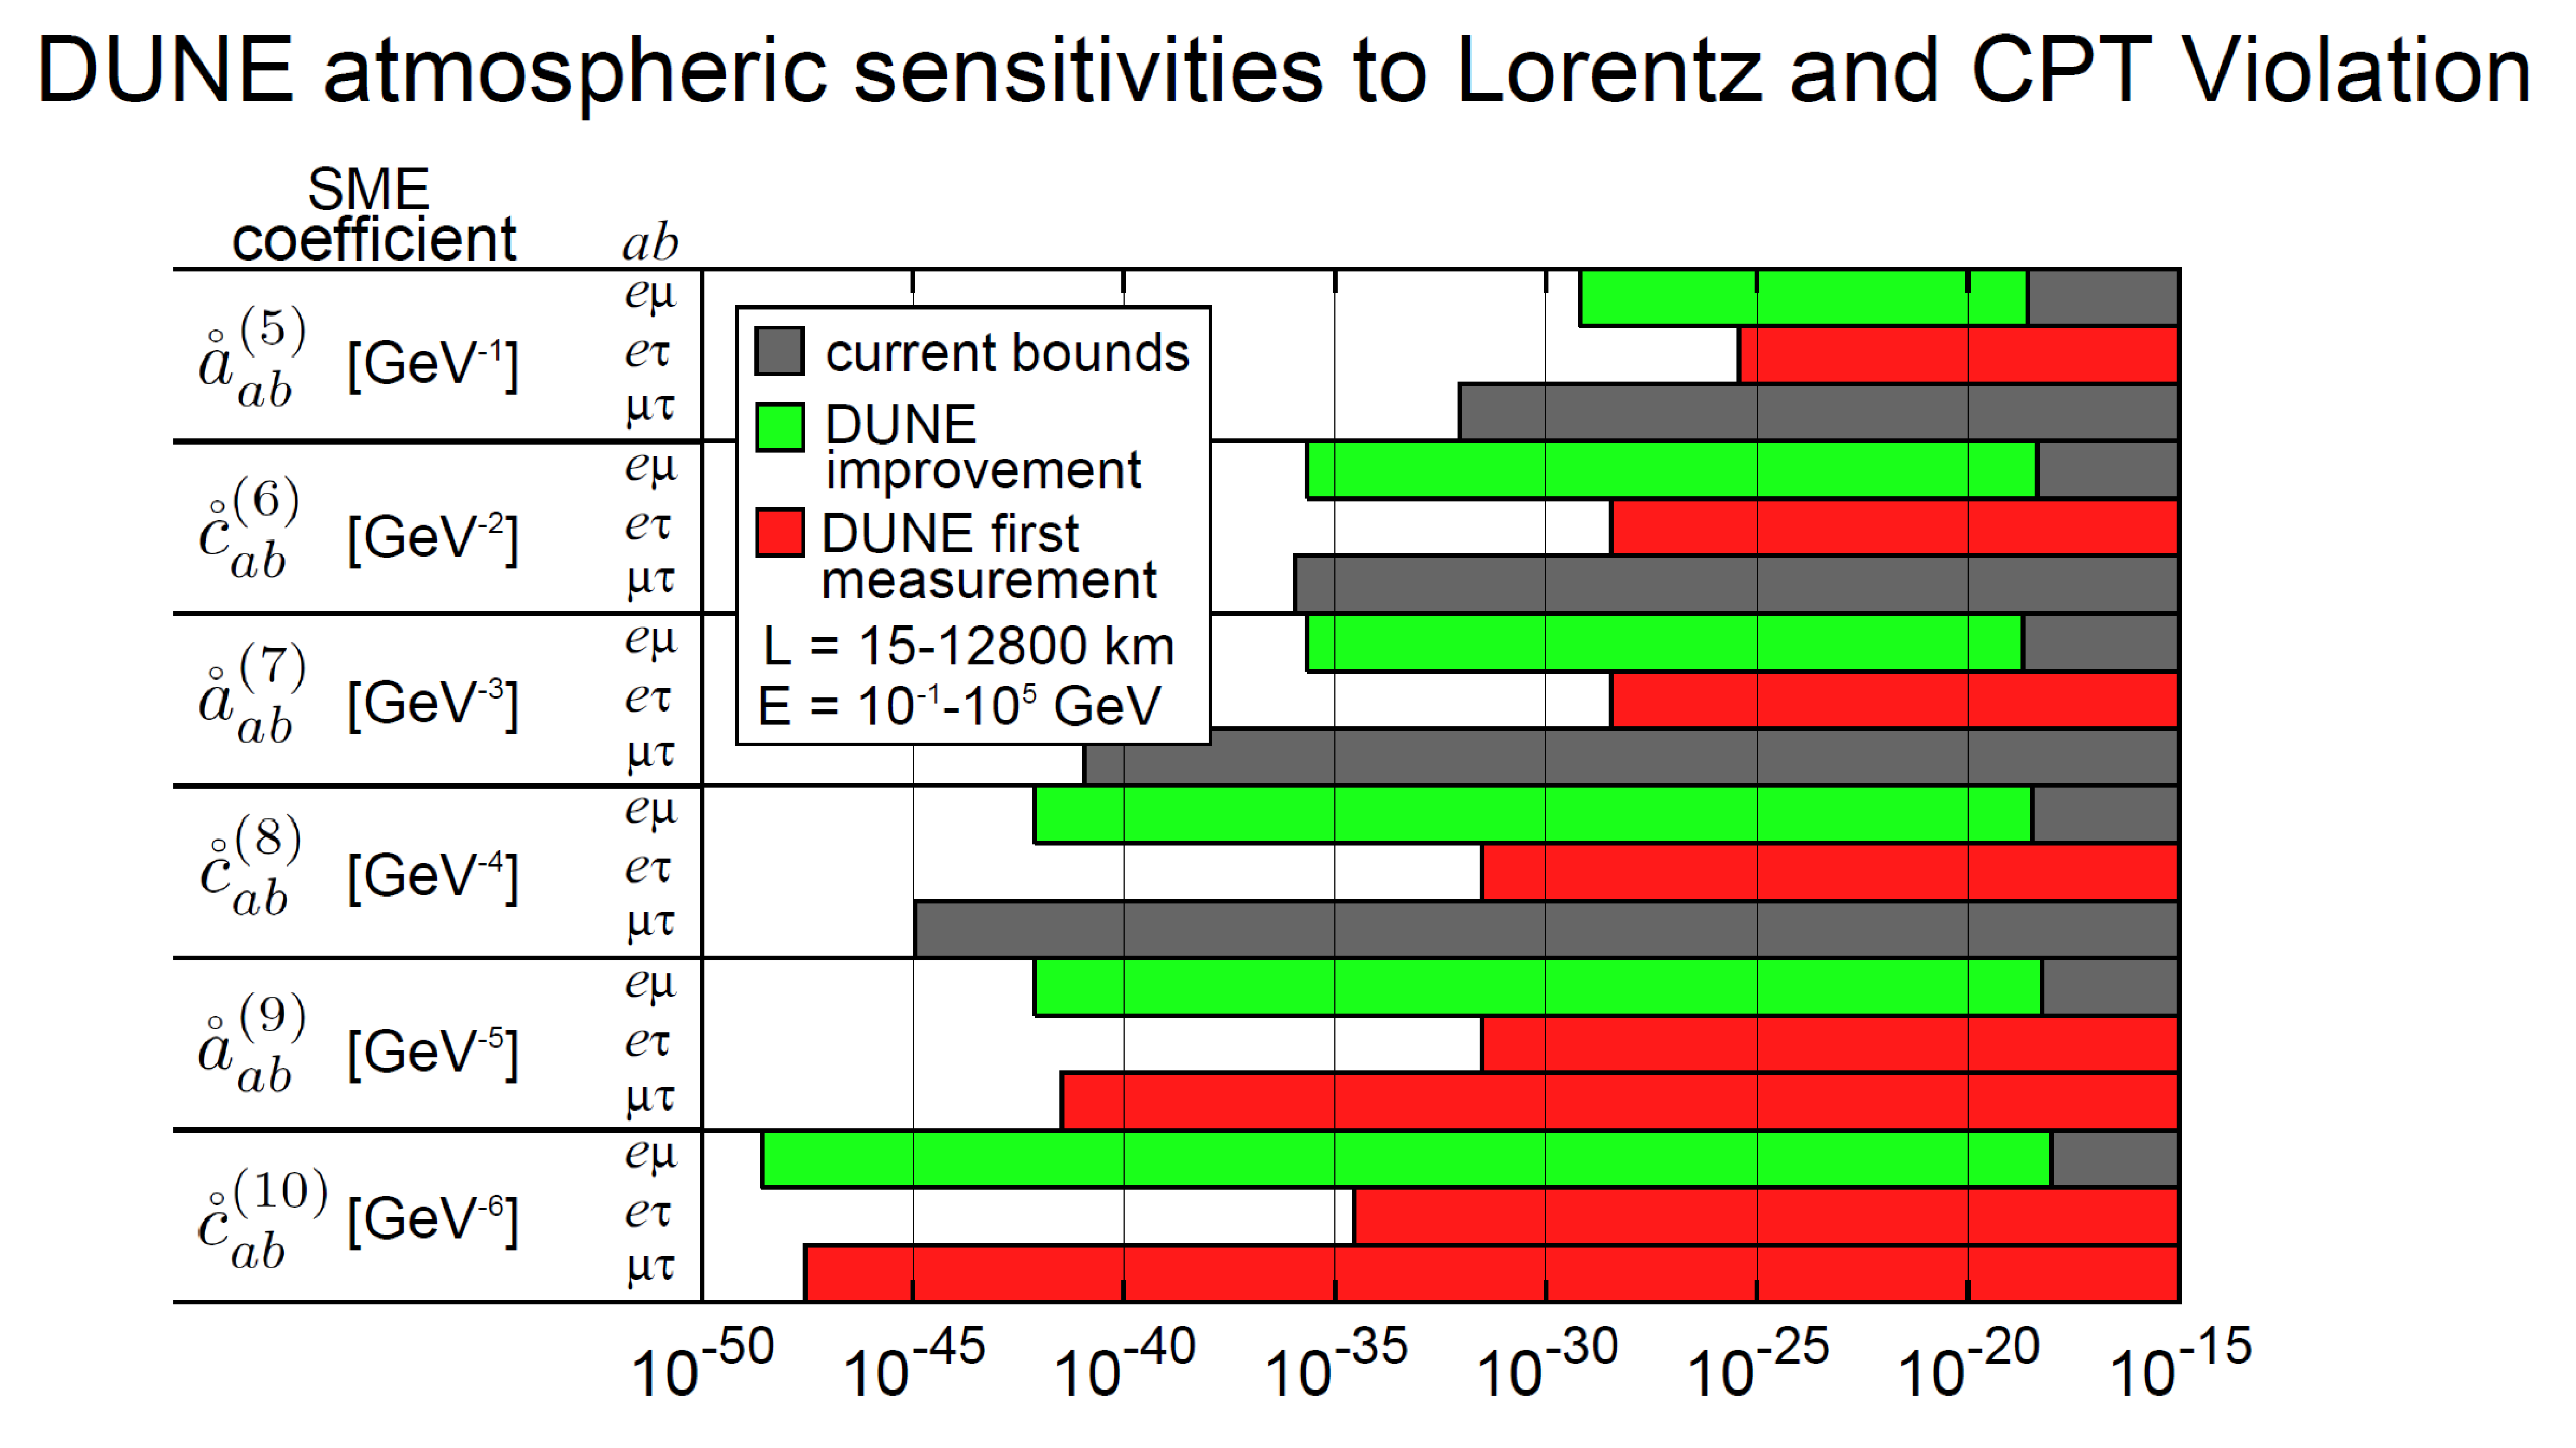
\includegraphics[width=0.8\textwidth]{DUNE-atm.pdf}
\end{dunefigure}

\begin{dunefigure}[Atmospheric $\nu$ and $\bar{\nu}$ fluxes in the non-minimal isotropic Standard Model Extension]{fig:atm2}{Atmospheric fluxes of neutrinos and antineutrinos as a function of energy for conventional oscillations (dashed line) and in the non-minimal isotropic Standard Model Extension (solid line).}
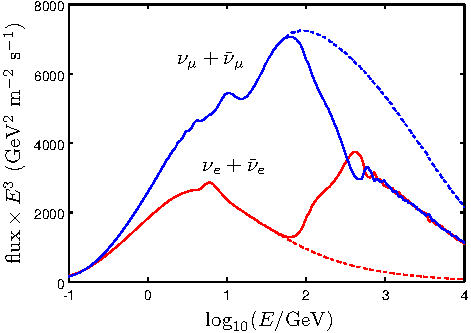
\includegraphics[width=0.8\textwidth]{DUNE-atm2.pdf}
\end{dunefigure}

%\subsection{Reconstruction of atmospheric neutrinos}
%\label{sec:nonaccel-atm-reco}

